\chapter{The SARS-CoV-2 receptor ACE2 in ME/CFS: A meta-analysis of public DNA methylation and gene expression data}
\chaptermark{The SARS-CoV-2 receptor ACE2 in ME/CFS}
\label{chapter:2021-ace-ace2}

%%%%%%%%%%%%%%%%%%%%%%%%%%%%%%%%%%%%%%%%%%%%%%%%%%%%%%%%%%%%%%%%%%%%%%%%
\noindent\underline{J. Malato}, F. Sotzny, S. Bauer, H. Freitag, A. Fonseca, A.D. Grabowska, L. Graça, C. Cordeiro, L. Nacul, E.M. Lacerda, J. Castro-Marrero, C. Scheibenbogen, F. Westermeier, and N. Sepúlveda. The SARS-CoV-2 receptor angiotensin-converting enzyme 2 (ACE2) in myalgic encephalomyelitis/chronic fatigue syndrome: A meta-analysis of public DNA methylation and gene expression data. \textit{Heliyon}. 2021; 7(8). doi: \url{https://doi.org/10.1016/j.heliyon.2021.e07665}.


%%%%%%%%%%%%%%%%%%%%%%%%%%%%%%%%%%%%%%%%%%%%%%%%%%%%%%%%%%%%%%%%%%%%%%%%
\begin{abstract}
People with myalgic encephalomyelitis/chronic fatigue syndrome (ME/CFS) often report a high frequency of viral infections and flu-like symptoms during their disease course. Given that this reporting agrees with different immunological abnormalities and altered gene expression profiles observed in the disease, we aimed at answering whether the expression of the human angiotensin-converting enzyme 2 (ACE2), the major cell entry receptor for SARS-CoV-2, is also altered in these patients. In particular, a low expression of ACE2 could be indicative of a high risk of developing Covid-19. We then performed a meta-analysis of public data on CpG DNA methylation and gene expression of this enzyme and its homologous ACE protein in peripheral blood mononuclear cells and related subsets. We found that patients with ME/CFS have decreased methylation levels of four CpG probes in the \textit{ACE} locus (cg09920557, cg19802564, cg21094739, and cg10468385) and of another probe in the promoter region of the \textit{ACE2} gene (cg08559914). We also found a decreased expression of \textit{ACE2} but not of \textit{ACE} in patients when compared to healthy controls. Accordingly, in newly collected data, there was evidence for a significant higher proportion of samples with an \textit{ACE2} expression below the limit of detection in patients than healthy controls. Altogether, patients with ME/CFS can be at a higher Covid-19 risk and, if so, they should be considered a priority group for vaccination by public health authorities. To further support this conclusion, similar research is recommended for other human cell entry receptors and cell types, namely, those cells targeted by the virus.
\keywords{Myalgic encephalomyelitis/Chronic fatigue syndrome; SARS-CoV-2; ACE2; Gene expression; DNA methylation}
\end{abstract}

%%%%%%%%%%%%%%%%%%%%%%%%%%%%%%%%%%%%%%%%%%%%%%%%%%%%%%%%%%%%%%%%%%%%%%%%
%%%%%%%%%%%%%%%%%%%%%%%%%%%%%%%%%%%%%%%%%%%%%%%%%%%%%%%%%%%%%%%%%%%%%%%%
%%%%%%%%%%%%%%%%%%%%%%%%%%%%%%%%%%%%%%%%%%%%%%%%%%%%%%%%%%%%%%%%%%%%%%%%
\section{Introduction}

Myalgic encephalomyelitis/Chronic fatigue syndrome (ME/CFS) is a multifactorial and complex disease characterised by two key symptoms: (1) persistent but unexplained fatigue that is not alleviated by rest; and (2) post-exertional malaise upon minimal physical or even mental effort \citep{fukuda1994ChronicFatigue, carruthers2003MyalgicEncephalomyelitis}. Although its cause remains unknown, a growing body of evidence strongly associates ME/CFS with several microbial and viral infections, as potential triggering factors \citep{chu2019OnsetPatterns, johnston2016EpidemiologicalCharacteristics}. In addition, it is currently hypothesised that reactivations of dormant viral infections also play a role \citep{rasa2018ChronicViral, ariza2021MyalgicEncephalomyelitis} due to several immunological abnormalities \citep{klimas1990ImmunologicAbnormalitiesa, lorussoImmunologicalAspectsChronic2009, brenuImmunologicalAbnormalitiesPotential2011}. On the molecular basis of the disease, peripheral blood mononuclear cells (PBMCs) have altered gene expression profiles \citep{kerr2008GeneExpression}, including a decreased abundance of the human angiotensin-converting enzyme 2 (ACE2) \citep{smithConvergentGenomicStudies2011}, the main receptor of the severe acute respiratory syndrome coronavirus-2 (SARS-CoV-2) for cell invasion \citep{li2003AngiotensinconvertingEnzyme, ge2013IsolationCharacterization, hoffmann2020SARSCoV2Cell}. Altogether, this evidence raises the question about the Covid-19 risk in patients with ME/CFS.

As basic information, ACE2 is encoded by the X-linked \textit{ACE2} gene whose expression is predominant in the lungs, heart, skin, and kidneys \citep{hamming2004TissueDistribution, to2004ExploringPathogenesis, li2020ExpressionSARSCoV2, radzikowska2020DistributionACE2}. Its expression can also be detected in monocytes \citep{rutkowska-zapala2015HumanMonocyte} and activated macrophages \citep{song2023LittleNo}. However, the percentage of \textit{ACE2}-expressing cells is below 5\% in the main immune-cell populations \citep{song2023LittleNo}. Accordingly, current RNA-Seq studies suggest a residual \textit{ACE2} expression in PBMCs from healthy controls \citep{radzikowska2020DistributionACE2}. ACE2 has an amino-acid sequence identity of 41\% with its homologous angiotensin-converting enzyme (ACE) \citep{tipnis2000HumanHomolog}. This sequence similarity increases to 61\% at the nucleotide level \citep{tipnis2000HumanHomolog}. The enzymes ACE and ACE2 are members of the renin-angiotensin-aldosterone system (RAAS), which regulates blood pressure and vascular resistance \citep{westermeier2015NovelPlayers}. In particular, ACE and ACE2 have vasoconstriction and vasodilation effects, respectively. Given this counteracting effect, high ACE:ACE2 ratios are possible indicators of severe Covid-19 outcomes, linked to increased reactive oxygen species (ROS) production, vasoconstriction, and inflammation \citep{pagliaro2020ACEACE2}.

To answer our research question, we performed a meta-analysis of public DNA methylation and gene expression data of \textit{ACE2} and \textit{ACE} in PBMCs. Similar study was conducted on the DNA methylation pattern of \textit{ACE2} in the same cell type from patients with systemic lupus erythematosus \citep{sawalha2020EpigeneticDysregulation}, an autoimmune disease whose symptoms overlap with the ones from ME/CFS \citep{blomberg2018InfectionEliciteda}. To complement our findings, we also compared the mRNA levels of these two genes in PBMCs from a new cohort of female patients with ME/CFS and healthy women.

%%%%%%%%%%%%%%%%%%%%%%%%%%%%%%%%%%%%%%%%%%%%%%%%%%%%%%%%%%%%%%%%%%%%%%%%
%%%%%%%%%%%%%%%%%%%%%%%%%%%%%%%%%%%%%%%%%%%%%%%%%%%%%%%%%%%%%%%%%%%%%%%%
%%%%%%%%%%%%%%%%%%%%%%%%%%%%%%%%%%%%%%%%%%%%%%%%%%%%%%%%%%%%%%%%%%%%%%%%
\section{Materials and methods}

%%%%%%%%%%%%%%%%%%%%%%%%%%%%%%%%%%%%%%%%%%%%%%%%%%%%%%%%%%%%%%%%%%%%%%%%
\subsection{Eligible diagnostic criteria of ME/CFS}

In our meta-analysis, we selected public data from studies using either the 1994 US Center for Disease Control and Prevention criteria (CDC-1994) \citep{fukuda1994ChronicFatigue} or the 2003 Canadian Consensus Criteria (CCC-2003) \citep{carruthers2003MyalgicEncephalomyelitis} for the disease diagnosis. These criteria are defined by the presence of several key symptoms while excluding known medical conditions (e.g., multiple sclerosis or lupus) that can also explain fatigue. The choice of using these two criteria for study selection complies with the research standards set by the European Network on ME/CFS \citep{pheby2020DevelopmentConsistent}.

%%%%%%%%%%%%%%%%%%%%%%%%%%%%%%%%%%%%%%%%%%%%%%%%%%%%%%%%%%%%%%%%%%%%%%%%
\subsection{Analysis of published DNA methylation association studies}

Our meta-analysis was based on six genome-wide DNA methylation association studies (Table~\ref{tab:methylation-studies}), four of which \citep{brenu2014MethylationProfile, vegaDNAMethylationModifications2014, vegaEpigeneticModificationsGlucocorticoid2017, trivedi2018IdentificationMyalgic} were previously reviewed \citep{almenar-perez2019EpigeneticComponents}, and other two published after this review \citep{herrera2018GenomeepigenomeInteractions, helliwell2020ChangesDNA}. Briefly, these studies aimed at identifying differentially methylated CpG dinucleotide sites between patients and healthy controls. Illumina methylation arrays were used to measure the respective DNA methylation levels with the exception of a single study (Table~\ref{tab:methylation-studies}). In this study, the measurements were made by the reduced representation bisulfite sequencing \citep{helliwell2020ChangesDNA}.

\begin{table}[h]
    \definecolor{MineShaft}{rgb}{0.121,0.121,0.121}
    \centering
    \caption[Summary of the six DNA methylation studies under analysis]{Summary of the six DNA methylation studies under analysis.}
    \resizebox{\textwidth}{!}{% \begin{tblr}{
%  column{1,4} = {l},
%  column{2,3,5-8} = {c},
%  cell{1}{1-2} = {r=2}{},
%  cell{1}{3} = {c=3}{},
%  cell{1}{6-8} = {r=2}{},
%  cell{3-8}{1} = {r=1}{},
%  hline{1,9} = {-}{0.08em},
%  hline{2} = {3-5}{0.03em},
%  hline{3} = {-}{0.05em},
% }
% Reference & Sample type & ME/CFS patients & & & {Healthy \\controls, $n$ } & {Technology \\(manufacturer) } & {NCBI GEO \\Accession \\ number } \\
%  & & $n$ & Sample characteristics & Case definition & & & \\
% \citet{brenu2014MethylationProfile} & CD4\textsuperscript{+} T cells & 25 & {Female/male adults\\Mean age: 50 years old\\Mean BMI: not reported} & CDC-1994 & 18 & {Infinium HumanMethylation450K\\Array (Illumina)} & --- \\
% \citet{vegaDNAMethylationModifications2014} & PBMC & 12 & {Female adults\\Mean age: 41 years old\\Mean BMI: 23 kg/m\textsuperscript{2}} & {CDC-1994 \&\\CCC-2003} & 12 & {Infinium HumanMethylation450K\\Array (Illumina)} & GSE59489 \\
% \citet{vegaEpigeneticModificationsGlucocorticoid2017} & PBMC & 49 & {Female adults\\Mean age: 50 years old\\Mean BMI: 23 kg/m\textsuperscript{2}} & {CDC-1994 \&\\CCC-2003} & 25 & {Infinium HumanMethylation450K\\Array (Illumina)} & GSE93266 \\
% \citet{trivedi2018IdentificationMyalgic} & PBMC & 13 & {Female adults\\Mean age: 50 years old\\Mean BMI: 26 kg/m\textsuperscript{2}} & {CDC-1994 \&\\CCC-2003} & 12 & Methylation EPIC Array (Illumina) & GSE111183 \\
% \citet{herrera2018GenomeepigenomeInteractions} & T lymphocytes & 61 & {Female/male adults\\Mean age: 32 years old\\Mean BMI: 27 kg/m\textsuperscript{2}} & {CDC-1994 \&\\CCC-2003} & 48 & {Infinium HumanMethylation450K\\Array (Illumina)} & GSE156792 \\
% \citet{helliwell2020ChangesDNA} & PBMC & 10 & {Female/male adults\\Mean age: not reported\\Mean BMI: not reported} & CCC-2003 & 10 & {Reduced representation\\Bisulfite sequencing} & GSE153667 
% \end{tblr}
\begin{tabular}{lcclcccc} 
\toprule
\multirow{2}{*}{Reference} & \multirow{2}{*}{Sample type} & \multicolumn{3}{c}{ME/CFS patients} & \multirow{2}{*}{\begin{tabular}[c]{@{}c@{}}Healthy\\controls,~$n$\end{tabular}} & \multirow{2}{*}{\begin{tabular}[c]{@{}c@{}}Technology\\(manufacturer)\end{tabular}} & \multirow{2}{*}{\begin{tabular}[c]{@{}c@{}}NCBI~GEO\\Accession number\end{tabular}}\\ 
\cmidrule{3-5}
 & & $n$ & Sample characteristics & Case definition & & & \\ 
\midrule
% 1
\citet{brenu2014MethylationProfile} & CD4\textsuperscript{+} T cells  & 25 & \begin{tabular}[c]{@{}l@{}}Female/male adults\\Mean age: 50 years old\\Mean BMI: not reported\end{tabular} & CDC-1994 & 18 & \begin{tabular}[c]{@{}c@{}}Infinium HumanMethylation450K\\Array (Illumina)\end{tabular} & NA \\
\midrule
% 2
\citet{vegaDNAMethylationModifications2014} & PBMC & 12 & \begin{tabular}[c]{@{}l@{}}Female adults\\Mean age: 41 years old\\Mean BMI: 23 kg/m\textsuperscript{2}\end{tabular} & \begin{tabular}[c]{@{}c@{}}CDC-1994 \&\\CCC-2003\end{tabular} & 12 & \begin{tabular}[c]{@{}c@{}}Infinium HumanMethylation450K\\Array (Illumina)\end{tabular} & GSE59489 \\
\midrule
% 3
\citet{vegaEpigeneticModificationsGlucocorticoid2017} & PBMC & 49 & \begin{tabular}[c]{@{}l@{}}Female adults\\Mean age: 50 years old\\Mean BMI: 23 kg/m\textsuperscript{2}\end{tabular} & \begin{tabular}[c]{@{}c@{}}CDC-1994 \&\\CCC-2003\end{tabular} & 25 & \begin{tabular}[c]{@{}c@{}}Infinium HumanMethylation450K\\Array (Illumina)\end{tabular} & GSE93266 \\
\midrule
% 4
\citet{trivedi2018IdentificationMyalgic} & PBMC & 13 & \begin{tabular}[c]{@{}l@{}}Female adults\\Mean age: 50 years old\\Mean BMI: 26 kg/m\textsuperscript{2}\end{tabular} & \begin{tabular}[c]{@{}c@{}}CDC-1994 \&\\CCC-2003\end{tabular} & 12 & Methylation EPIC Array (Illumina) & GSE111183 \\
\midrule
% 5
\citet{herrera2018GenomeepigenomeInteractions} & T lymphocytes & 61 & \begin{tabular}[c]{@{}l@{}}Female/male adults\\Mean age: 32 years old\\Mean BMI: 27 kg/m\textsuperscript{2}\end{tabular} & \begin{tabular}[c]{@{}c@{}}CDC-1994 \&\\CCC-2003\end{tabular} & 48 & \begin{tabular}[c]{@{}c@{}}Infinium HumanMethylation450K\\Array (Illumina)\end{tabular} & GSE156792 \\
\midrule
% 6
\citet{helliwell2020ChangesDNA} & PBMC & 10 & \begin{tabular}[c]{@{}l@{}}Female/male adults\\Mean age: not reported\\Mean BMI: not reported\end{tabular} & CCC-2003 & 10 & \begin{tabular}[c]{@{}c@{}}Reduced representation\\Bisulfite sequencing\end{tabular} & GSE153667 \\
\bottomrule
\end{tabular}}
    \label{tab:methylation-studies}
\end{table}
% Table 1
% Table~\ref{tab:methylation-studies}

With respect to the exclusion criteria, one study excluded individuals who were taking beta-blockers or ACE inhibitors \citep{trivedi2018IdentificationMyalgic}. Three studies excluded participants who were treated with immunomodulatory effects or affecting the underlying DNA methylation levels at the time of data collection \citep{vegaDNAMethylationModifications2014, vegaEpigeneticModificationsGlucocorticoid2017, herrera2018GenomeepigenomeInteractions}.

In four of the published DNA methylation studies, patients and healthy controls were matched for age, gender, and body mass index (Table~\ref{tab:methylation-studies}) \citep{vegaDNAMethylationModifications2014, vegaEpigeneticModificationsGlucocorticoid2017, trivedi2018IdentificationMyalgic}. In two other studies, the matching was only based on age and gender \citep{brenu2014MethylationProfile, helliwell2020ChangesDNA}. Ethnicity was also used for further matching \citep{trivedi2018IdentificationMyalgic, herrera2018GenomeepigenomeInteractions} or the same matching could be assumed in studies that only recruited white females \citep{vegaDNAMethylationModifications2014, vegaEpigeneticModificationsGlucocorticoid2017}. The DNA methylation levels were quantified in CD4\textsuperscript{+} T cells \citep{brenu2014MethylationProfile}, PBMCs \citep{vegaDNAMethylationModifications2014, vegaEpigeneticModificationsGlucocorticoid2017, trivedi2018IdentificationMyalgic, helliwell2020ChangesDNA}, and T lymphocytes \citep{herrera2018GenomeepigenomeInteractions}.

We conducted a joint analysis of the four array-based studies which made the data available \citep{vegaDNAMethylationModifications2014, vegaEpigeneticModificationsGlucocorticoid2017, trivedi2018IdentificationMyalgic, herrera2018GenomeepigenomeInteractions}. We first retrieved the data from all the CpG probes located in the coding regions and the transcription starting sites (TSS) of \textit{ACE} and \textit{ACE2}, respectively. We then restricted our data analysis to the 27 probes shared between the Infinium HumanMethylation450K and the Infinium HumanMethylationEPIC arrays (Supplementary Table~\ref{appendix:taba1-ace-ace2-cpg-probes}).

Before conducting the statistical analysis itself, we checked whether (1) the selected probes showed a high probability of detection, (2) they were not cross-reactive with other genomic regions, and (3) they were not affected by single nucleotide polymorphisms (SNPs) with high minor allele frequencies \citep{dedeurwaerder2014ComprehensiveOverview}. In the latter criterion, the SNPs included in the selected probes had a minor allele frequency less than 5\% in Europeans and North Americans (Figure~\ref{fig:dna-methylation-analysis}A; Supplementary Table~\ref{appendix:taba2-ace-ace2-cpg-polymorphic-probes}) referring to the sampled populations of the studies. All probes passed the remaining basic quality control checks.

\begin{figure}
    \centering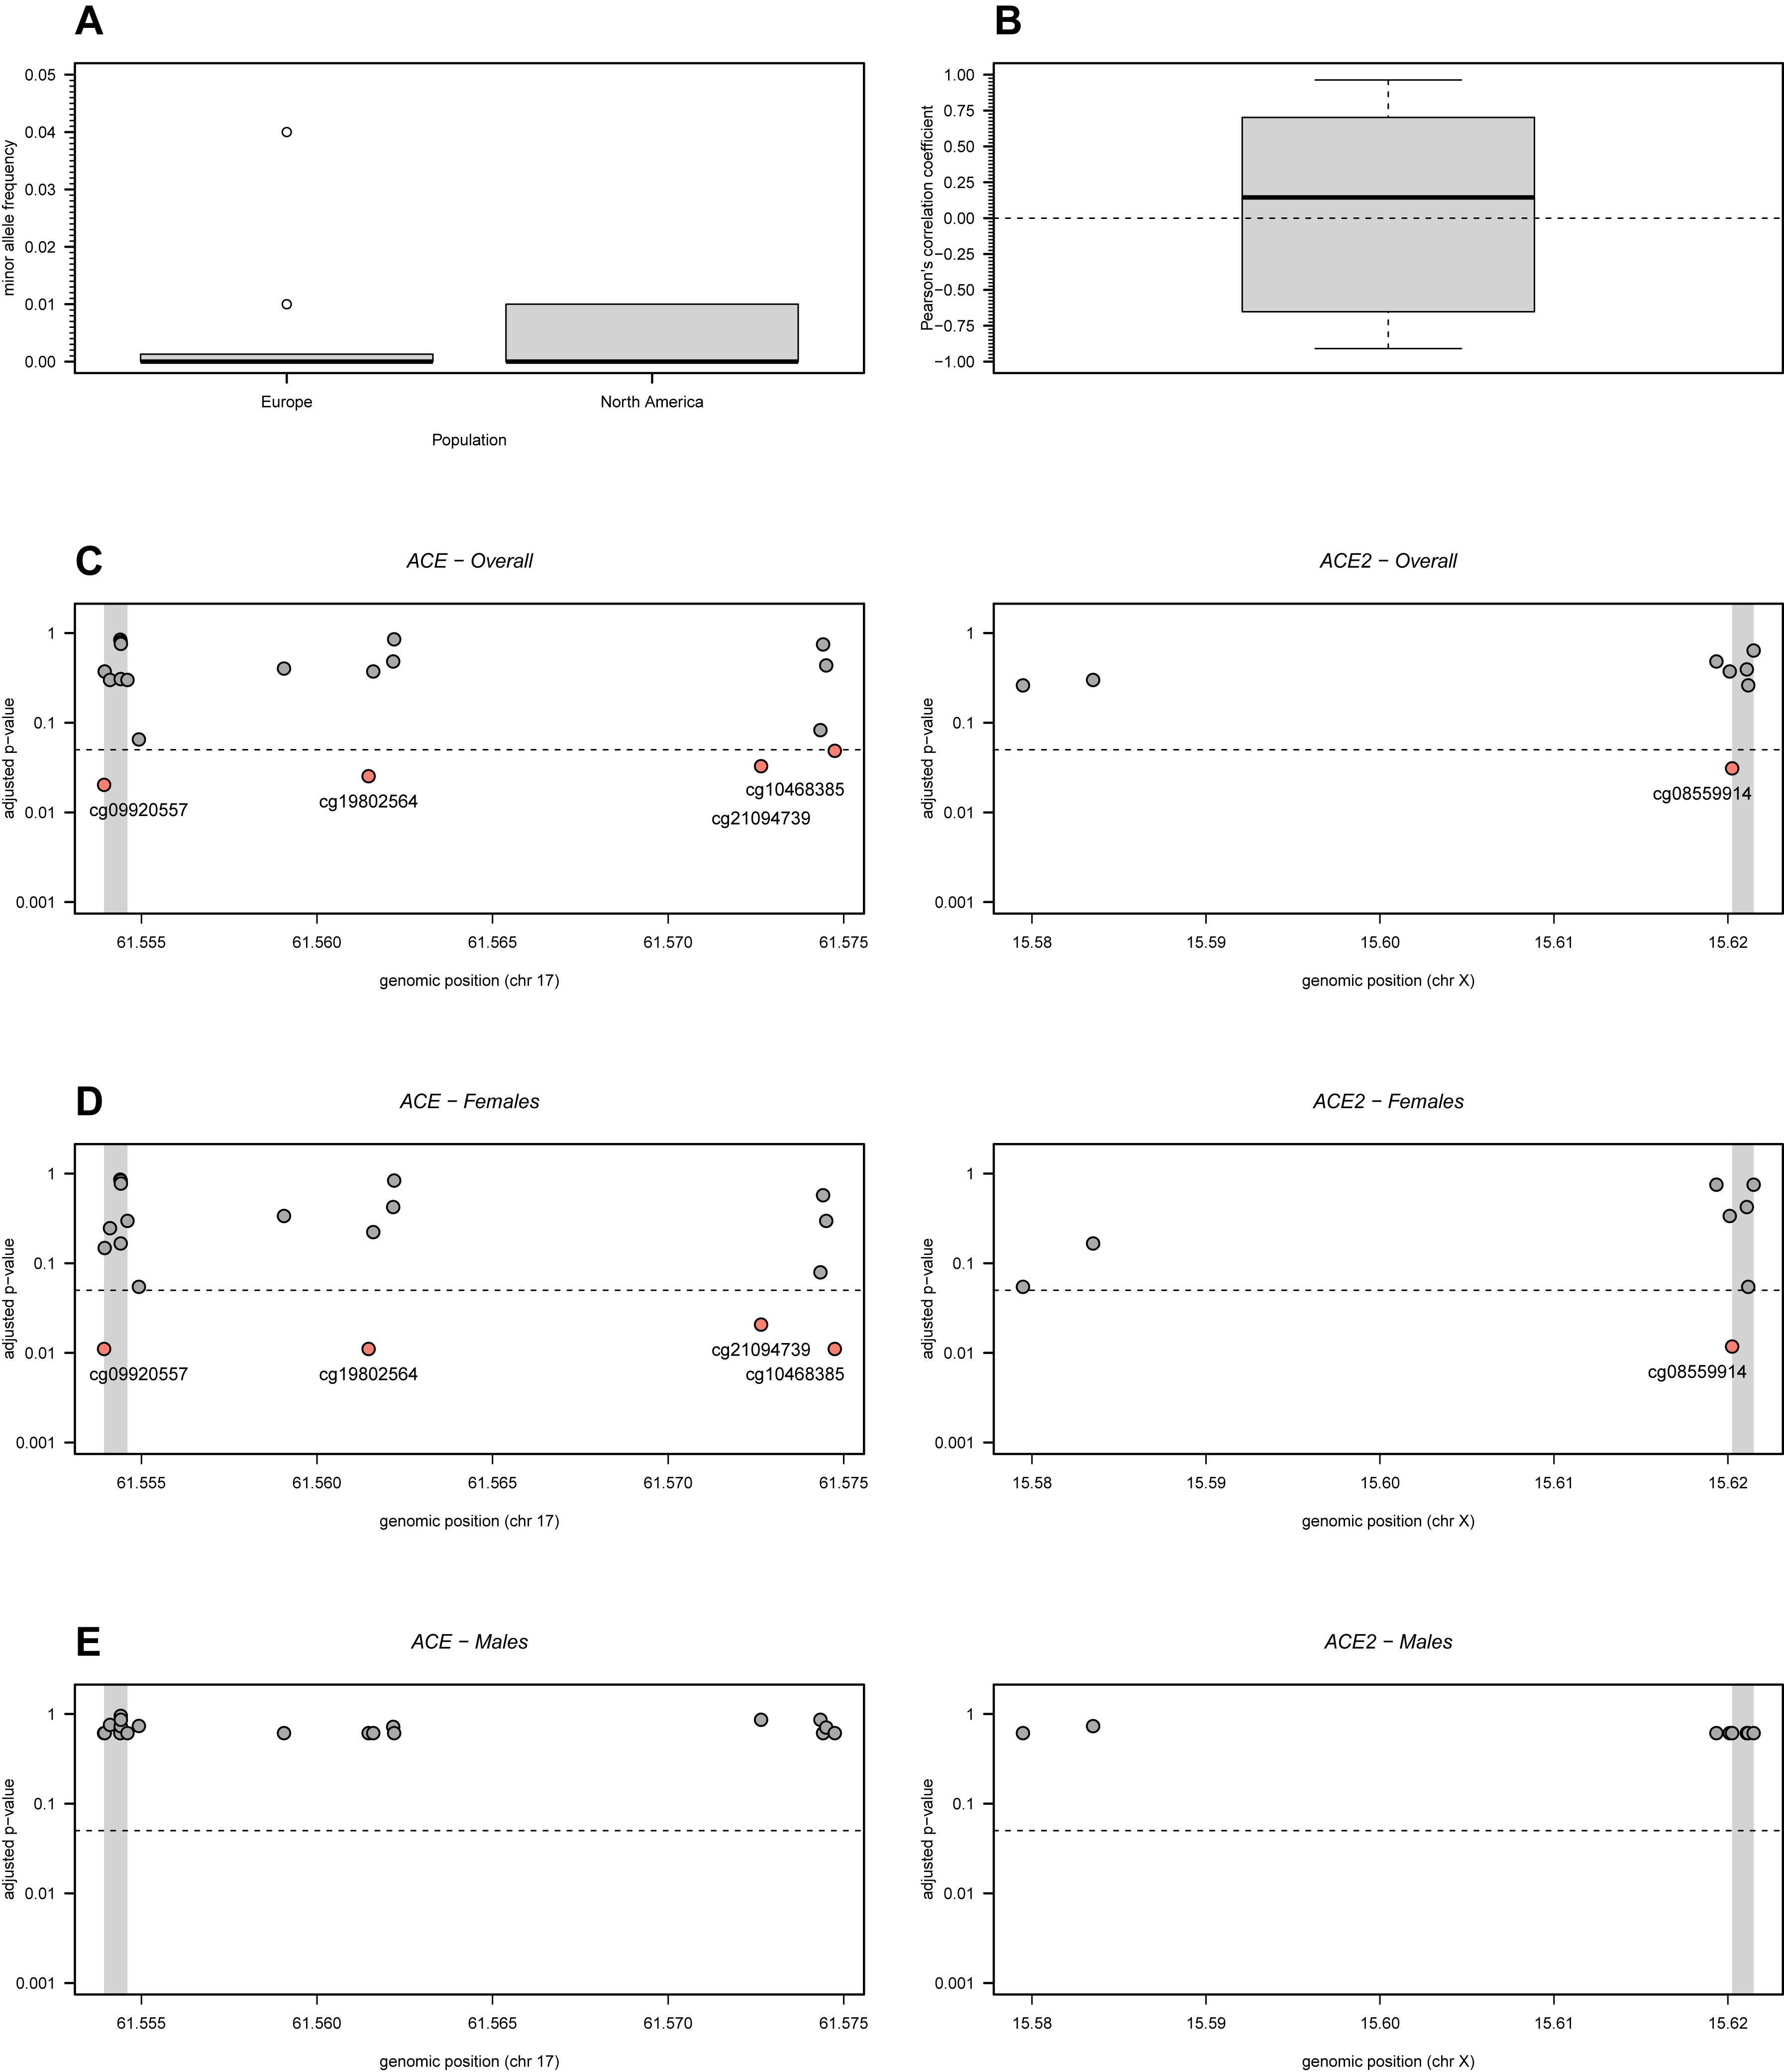
\includegraphics[width=0.9\textwidth]{chapter/2021-ace-ace2/figures/fig1-dna-methylation-analysis.jpg}
    \caption[DNA methylation analysis of 19 and 8 CpG probes located in the \textit{ACE} and \textit{ACE2} genes, respectively]{DNA methylation analysis of 19 and 8 CpG probes located in the \textit{ACE} and \textit{ACE2} genes, respectively. (A) Minor allele frequency in European and North American populations of SNPs located in the probes under analysis (see the respective data in Supplementary Table~\ref{appendix:taba2-ace-ace2-cpg-polymorphic-probes}). (B) Boxplot of all possible Pearson's correlation coefficients ($y$ axis) between the M-values of the probes under analysis. Horizontal dashed line represents the situation of lack of correlation. (C) Adjusted p-values for the overall association between each probe and ME/CFS. Adjusted p-values were calculated according to the Benjamini-Hochberg procedure with a false discovery rate of 5\% (dashed line). Grey areas in the plots represent the TSS of the genes. (D) and (E) The same analyses as shown in C but for women and men separately.}
    \label{fig:dna-methylation-analysis}
\end{figure}
% Figure 1
% Figure~\ref{fig:dna-methylation-analysis}

We analysed the M-values of a given probe instead of the respective $\beta$-values to ensure a good approximation of the Normal distribution to the data \citep{du2010ComparisonBetavalue}. Briefly, the $\beta$-values were calculated as the proportion of the methylation signal relative to the total signal for a given probe. The M-values were finally obtained by applying a logit transformation to the $\beta$-values.

To analyse the M-values of each probe, we initially estimated a linear regression model where the respective covariates were the study indicator and the disease status of the participants. In this model, we included the main effects of the covariates and the interaction. The model parameters were then estimated by the maximum likelihood method. Note that the main effect of the disease status is usually seen as the pooled effect of this covariate across all studies, as done in meta-analysis.

We then simplified the model using a backward stepwise procedure based on Akaike's information criteria. Since the effect of the study indicator was significant for the data of each probe, we tested the association between ME/CFS and a given probe using a likelihood ratio test. In this test, we compared the model including the study indicator only with the best model including that covariate and the one associated with disease status (i.e., either the model only including the main effects or the model including both main effects and the interaction term).

To control for multiple testing, we adjusted the raw p-values using the Benjamini-Hochberg procedure \citep{benjaminiControllingFalseDiscovery1995}. This adjustment ensured a false discovery rate of 5\% under the assumption of independent tests. Pearson's correlation coefficient was used to check the validity of this assumption (Figure~\ref{fig:dna-methylation-analysis}B).

We also repeated the same association analysis for women and men separately. Note that three studies only recruited women \citep{vegaDNAMethylationModifications2014, vegaEpigeneticModificationsGlucocorticoid2017, trivedi2018IdentificationMyalgic} while the remaining study recruited both men and women \citep{herrera2018GenomeepigenomeInteractions}. In the latter study, there was no information available about the gender of each participant. In this case, we estimated this missing information using the function \textit{getSex} of the R package \textit{minfi} applied to the genome-wide DNA methylation data \citep{aryee2014MinfiFlexible}. The resulting frequencies of men and women matched with those reported in the original study.

In the women-specific analysis, we performed the same association analysis as described above. In the men-specific analysis, we compared a linear regression model with the disease status as the single covariate against another model without that covariate, when analysing data from each probe. The comparison was done by the likelihood ratio test whose p-values were then adjusted for multiple testing in the same way as described above.

Finally, for the study which did not share the respective data \citep{brenu2014MethylationProfile}, we checked whether the reported differentially methylated CpG probes were located in either \textit{ACE} or \textit{ACE2} (see Table~1 from this study). We did the same for the study based on the reduced representation bisulfite sequencing technology \citep{helliwell2020ChangesDNA} (see Additional File 1 from this study).

%%%%%%%%%%%%%%%%%%%%%%%%%%%%%%%%%%%%%%%%%%%%%%%%%%%%%%%%%%%%%%%%%%%%%%%%
\subsection{Analysis of gene expression studies}

Our meta-analysis of gene expression studies was focused on eight reports using microarray technology (Table~\ref{tab:microarray-studies}) \citep{whistlerExerciseResponsiveGenes2005, kaushik2005GeneExpression, kerr2008GeneExpression, saikiIdentificationMarkerGenes2008, pietrangelo2009TranscriptionProfile, gowGeneSignaturePostinfectious2009, smithConvergentGenomicStudies2011, jeffreyTreatmentAvenuesMyalgic2019}. These studies complied with the Minimum Information about a Microarray Experiment (MIAME) standard \citep{brazma2001MinimumInformation} and, therefore, they were considered to have sufficient quality for their inclusion in the meta-analysis. In particular, these studies normalised the data which ensured comparability between different samples and between different measurements of the same genes.

\begin{table}[h]
    \centering
    \caption[Summary of the 8 microarray-based gene expression studies under analysis]{Summary of the 8 microarray-based gene expression studies under analysis, ordered by the year of publication.}
    \resizebox{\textwidth}{!}{\begin{tabular}{lcclccccc} 
\toprule
\multirow{2}{*}{Reference} & \multirow{2}{*}{Sample type} & \multicolumn{3}{c}{ME/CFS patients} & \multirow{2}{*}{\begin{tabular}[c]{@{}c@{}}Healthy \\controls,~$n$\end{tabular}} & \multirow{2}{*}{\begin{tabular}[c]{@{}c@{}}Technology \\(manufacturer)\end{tabular}} & \multirow{2}{*}{\begin{tabular}[c]{@{}c@{}}ACE/ACE2\\available\end{tabular}} & \multirow{2}{*}{\begin{tabular}[c]{@{}c@{}}Data availability\\(NCBI GEO\\Assession number)\end{tabular}} \\ 
\cmidrule{3-5}
 & & $n$ & Sample characteristics & Case definition & & & & \\ 
\midrule
% 1
\citet{whistlerExerciseResponsiveGenes2005} & PBMC & 5 & \begin{tabular}[c]{@{}l@{}}Female adults\\Mean age: 42 years old\\Mean BMI: not reported\end{tabular} & CDC-1994 & 5 & \begin{tabular}[c]{@{}c@{}}Atlas Glass\\Human 3.8 I Microarray\\(BD Biosciences Clontech)\end{tabular} & No/No & No (NA) \\
\midrule
% 2
\citet{kaushik2005GeneExpression} & PBMC & 25 & \begin{tabular}[c]{@{}l@{}}Female/male adults\\Mean age: 41 years old\\Mean BMI: not reported\end{tabular} & CDC-1994 & 25 & \begin{tabular}[c]{@{}c@{}}Custom microarray\\(Nimblegen)\end{tabular} & Unclear & No (NA) \\
\midrule
% 3
\citet{kerr2008GeneExpression} & Whole blood & 25 & \begin{tabular}[c]{@{}l@{}}Female/male adults\\Mean age: 43 years old\\Mean BMI: not reported\end{tabular} & CDC-1994 & 50 & \begin{tabular}[c]{@{}c@{}}GeneChip\\Human Genome\\U133 Plus 2.0\\(Affymetrix)\end{tabular} & Yes/Yes & No (NA) \\
\midrule
% 4
\citet{saikiIdentificationMarkerGenes2008} & Whole blood & 11 & \begin{tabular}[c]{@{}l@{}}Female/male adults\\Mean age: 34 years old\\Mean BMI: 20.3 kg/m\textsuperscript{2}\end{tabular} & CDC-1994 & 11 & \begin{tabular}[c]{@{}c@{}}Custom\\microarray (NA)\end{tabular} & Yes/No & Yes (NA){$^1$} \\
\midrule
% 5
\citet{pietrangelo2009TranscriptionProfile} & Muscle biopsies & 4 & \begin{tabular}[c]{@{}l@{}}Female/male adults\\Mean age: 45/37 years old\\Mean BMI: not reported\end{tabular} & CDC-1994 & 5 & \begin{tabular}[c]{@{}c@{}}Operon V2.0\\(CRIBI\\University of Padova)\end{tabular} & Yes/Yes & No (NA) \\
\midrule
% 6
\citet{gowGeneSignaturePostinfectious2009} & PBMC & \multicolumn{1}{l}{8} & \begin{tabular}[c]{@{}l@{}}Male adults\\Median age: 36 years old\\Mean BMI: not reported\end{tabular} & CDC-1994 & 7 & \begin{tabular}[c]{@{}c@{}}GeneChip\\Human Genome\\U133 (Affymetrix)\end{tabular} & Yes/Yes & Yes (GSE14577) \\
\midrule
% 7
\citet{smithConvergentGenomicStudies2011} & PBMC & \multicolumn{1}{l}{37} & \begin{tabular}[c]{@{}l@{}}Female/male adults\\Mean age: 51 years old\\Mean BMI:29.4 kg/m\textsuperscript{2}\end{tabular} & CDC-1994 & 25 & \begin{tabular}[c]{@{}c@{}}MWG 20K\\human Array\\(Biotech MWG)\end{tabular} & Yes/Yes & No (NA) \\
\midrule
% 8
\citet{jeffreyTreatmentAvenuesMyalgic2019} & PBMC & 33 & \begin{tabular}[c]{@{}l@{}}Female/male adults\\Mean age: not reported\\Mean BMI: not reported\end{tabular} & CDC-1994 & 21 & \begin{tabular}[c]{@{}c@{}}GeneChip\\Human Gene\\ST (Affymetrix)\end{tabular} & Yes/No & No (NA) \\
\bottomrule
\end{tabular}}
    \label{tab:microarray-studies}
    \raggedright{\scriptsize $^1$Data shared as a supplementary file in the online version of the study.}
\end{table}
% Table 2
% Table~\ref{tab:microarray-studies}

Gene expression of these studies was performed in PBMCs (5 studies), whole blood (2 studies) and muscle biopsies (one study). One study excluded participants who were taking any regular medication \citep{gowGeneSignaturePostinfectious2009}. Another study reviewed the medications taken by the participants \citep{smithConvergentGenomicStudies2011}. However, it was unclear which medications were considered as a part of the exclusion criteria. A third study reported that healthy controls were free from any medication at the time of sampling \citep{saikiIdentificationMarkerGenes2008}.

Three additional studies using microarray technology \citep{vernon2002UtilityBlood, galbraith2011PeripheralBlood, nguyen2017WholeBlood} were excluded from our meta-analysis due to unclear or ineligible case definitions of ME/CFS. We also excluded four RNA-seq studies \citep{bouquetRNASeqAnalysisGene2017, bouquetWholeBloodHuman2019, sweetman2019ChangesTranscriptome, raijmakersPossibleRoleMitochondrialderived2019}, because of insufficient reporting on the basic quality control checks. In particular, these studies did not report the percentage of reads that could be mapped onto the reference transcriptome, the percentage of the transcriptome covered, the average number of mapped reads per transcript, the relationship between the GC content and the mapped read distribution, as recommended elsewhere \citep{conesa2016SurveyBest}. More importantly, given the high sequence homology between ACE and ACE2, these studies did not explain how their mapping algorithms dealt with reads that could be ambiguously mapped onto different locations in the transcriptome.

The selected studies were conducted in small cohorts of patients with ME/CFS (mean sample size $=$ 18.5; range $=$ 4--37) and healthy controls (mean sample size $=$ 18.6; range $=$ 5--50 individuals) (Table~\ref{tab:microarray-studies}). In these studies, the patients and healthy controls were matched for age and gender. Different commercial and custom microarray technologies were used for the respective gene expression quantification. There was only one study in which the microarray did not include any probe in the genes of interest \citep{whistlerExerciseResponsiveGenes2005}. Another study used a custom array based on 9,522 genes from the RefSeq database, as available in August 2002 \citep{kaushik2005GeneExpression}. However, this study did not provide the list of genes included in the respective microarray. In terms of data sharing, one study made the data available in the GEO database \citep{gowGeneSignaturePostinfectious2009} and another one within the respective publication \citep{saikiIdentificationMarkerGenes2008}. The latter study used a custom microarray that measured the expression of stress-related genes including \textit{ACE} but excluding \textit{ACE2}.

Before conducting a meta-analysis of the available data, we first re-analysed two studies where the normalized data were available \citep{saikiIdentificationMarkerGenes2008, gowGeneSignaturePostinfectious2009}. In the first study \citep{saikiIdentificationMarkerGenes2008}, we calculated the mean of the {$\log_{2}$}(fold-change) for \textit{ACE} and the respective standard error. Note that the microarray used in this study did not include any probe in \textit{ACE2}. In the second study \citep{gowGeneSignaturePostinfectious2009}, we initially calculated the mean and the respective standard error of the {$\log_{2}$}(fold-change) for each probe located in \textit{ACE} and \textit{ACE2}. We then pooled each pair of means for the same gene using the inverse-variance weighting method \citep{hartung2008StatisticalMeta}. A third study reported the mean of the {$\log_{2}$}(fold-change) for \textit{ACE2} and the respective p-value using a two-tailed Student's test \citep{smithConvergentGenomicStudies2011}. In this case, we determine the quantile of the t-distribution associated with half of the reported p-value, equated it to the test statistic, and solved the resulting equation as a function of the standard error. No information was available from this study concerning the expression levels of \textit{ACE}.

Finally, we pooled the different estimates for the same gene from different studies using the inverse-variance weighting method \citep{hartung2008StatisticalMeta}.

%%%%%%%%%%%%%%%%%%%%%%%%%%%%%%%%%%%%%%%%%%%%%%%%%%%%%%%%%%%%%%%%%%%%%%%%
\subsection{Analysis of new RNA data on the ACE/ACE2 gene expression in ME/CFS}

%%%%%%%%%%%%%%%%%%%%%%%%%%%%%%%%%%%%%%%%%%%%%%%%%%%%%%%%%%%%%%%%%%%%%%%%
\subsubsection{Study participants}

Thirty-seven women with ME/CFS were recruited in 2020 from the outpatient clinic for immunodeficiencies at the Institute for Medical Immunology at the Charité-Universitätsmedizin Berlin, Germany. These patients were diagnosed according to the CCC-2003 while excluding other medical or neurological diseases which could explain fatigue \citep{carruthers2003MyalgicEncephalomyelitis}. Thirty-four women with self-reported healthy status were recruited from staff.

%%%%%%%%%%%%%%%%%%%%%%%%%%%%%%%%%%%%%%%%%%%%%%%%%%%%%%%%%%%%%%%%%%%%%%%%
\subsubsection{Experimental procedure for RNA isolation and expression}

Consistently with previous studies of ME/CFS, the gene expression quantification was performed in PBMCs. These cells were isolated from heparinized whole blood by density gradient centrifugation using Biocoll Separating Solution (Merck Millipore). Total RNA was isolated and extracted from $2\times10^6$ PBMCs according to the manufacturer's instructions (NucleoSpin RNA Kit, Macherey-Nagel, cat. nr. 740955.50). Afterwards cDNA was prepared by reverse transcription (High-Capacity cDNA Reverse Transcription Kit, Applied Biosystems, cat. nr. 4368814) and real-time PCR was performed using TaqMan\textsuperscript{\texttrademark} Universal PCR Master Mix (cat. nr. 4305719) and TaqMan\textsuperscript{\texttrademark} Gene Expression Assays (cat. nr. 4331182) for \textit{ACE} (Hs00174179\_m1), \textit{ACE2} (Hs01085333\_m1) and the housekeeping gene \textit{HPRT1} (Hs02800695\_m1) (Applied Biosystems). The amplification of \textit{ACE} and \textit{HPRT1} was based on 20 ng template cDNA. For the amplification of \textit{ACE2}, this quantity was increased to 100 ng. All measurements were performed with the ABI7200 and software Step One Plus as absolute quantification according to manufacturer's instruction. Relative gene expression was analysed using the ${\Delta}$CT method.

%%%%%%%%%%%%%%%%%%%%%%%%%%%%%%%%%%%%%%%%%%%%%%%%%%%%%%%%%%%%%%%%%%%%%%%%
\subsubsection{Statistical analysis}

We first tested whether patients and healthy controls were matched for age using the Kolgomorov-Smirnov test for two independent samples. For statistical convenience, gene expression values were independently transformed for ACE and ACE2 using a Box-Cox transformation \citep{asar2017EstimatingBoxCox}. The parameter estimates of this transformation were 0.303 and 0.225 for ACE and ACE2, respectively. The transformed values for each gene were then analysed as the outcome variable of a linear regression model specifying age and disease status of the participants as the respective covariates. The linear regression model was estimated using the maximum likelihood method. After estimating the models, we tested the Normal distribution in the resulting residuals using the Shapiro-Wilk test. We also visually inspected the assumption of constant variance of the same residuals as a function of the covariates.

Note that we were unable to quantify the \textit{ACE2} expression in 11 patients due to cDNA material below the limit of detection. These problematic samples could be due to a lower expression of \textit{ACE2} in ME/CFS patients than in healthy controls. To test this hypothesis, we compared the respective proportion of samples below the limit of detection using the Pearson's $\chi^2$ test for two-way frequency tables.
The significance level of the statistical analysis was set at 5\%.

%%%%%%%%%%%%%%%%%%%%%%%%%%%%%%%%%%%%%%%%%%%%%%%%%%%%%%%%%%%%%%%%%%%%%%%%
\subsubsection{Ethical approval}

The protocol of this study was approved by the Ethics Committee of Charité-Universitätsmedizin Berlin in accordance with the 1964 Declaration of Helsinki and its later amendments (reference number EA2/067/20). All patients and healthy controls gave written informed consent to participate in the study.

%%%%%%%%%%%%%%%%%%%%%%%%%%%%%%%%%%%%%%%%%%%%%%%%%%%%%%%%%%%%%%%%%%%%%%%%
\subsection{Statistical software}

We performed our statistical analysis in the R software version 4.0.3. In this analysis, we used the following Bioconductor packages: \textit{hgu133a.db}, \textit{hgu133plus2.db}, \textit{IlluminaHumanMethylation450kanno.ilmn12.hg19}, and \textit{IlluminaHumanMethylationEPICanno.ilm10b2.hg19} to retrieve the annotation of the GeneChip HG-U133A, GeneChip U133+2, Infinium HumanMethylation450K Array and HumanMethylationEPIC arrays, respectively; \textit{minfi} to estimate the sex of each individual from DNA methylation data \citep{aryee2014MinfiFlexible}. The R scripts are freely available from the first and last authors upon request.

%%%%%%%%%%%%%%%%%%%%%%%%%%%%%%%%%%%%%%%%%%%%%%%%%%%%%%%%%%%%%%%%%%%%%%%%
%%%%%%%%%%%%%%%%%%%%%%%%%%%%%%%%%%%%%%%%%%%%%%%%%%%%%%%%%%%%%%%%%%%%%%%%
%%%%%%%%%%%%%%%%%%%%%%%%%%%%%%%%%%%%%%%%%%%%%%%%%%%%%%%%%%%%%%%%%%%%%%%%
\section{Results}

%%%%%%%%%%%%%%%%%%%%%%%%%%%%%%%%%%%%%%%%%%%%%%%%%%%%%%%%%%%%%%%%%%%%%%%%
\subsection{Meta-analysis of ACE/ACE2 DNA methylation in ME/CFS patients}

The oldest DNA methylation study \citep{brenu2014MethylationProfile} did not make the data available and hence, we screened the list of 120 differentially methylated probes (see Table 1 from this study). Although located in 70 genes, these probes were neither located in \textit{ACE} nor \textit{ACE2}. We also screened the list of differentially methylated probes reported by the study based on the reduced representation bisulfite sequencing technology (see Additional File 1 from \citet{helliwell2020ChangesDNA}). Again, none of these probes was in the ACE or ACE2 loci.

For the four array-based studies \citep{vegaDNAMethylationModifications2014, vegaEpigeneticModificationsGlucocorticoid2017, trivedi2018IdentificationMyalgic, herrera2018GenomeepigenomeInteractions}, we conducted a joint analysis of the respective data in accordance with a meta-analysis. We first observed that the M-values of the 27 probes under investigation tended to be uncorrelated with each other (Figure~\ref{fig:dna-methylation-analysis}B). This observation supported the use of the Benjamini-Hochberg procedure to adjust the raw p-values under a multiple testing scenario.

The subsequent analysis suggested four CpG probes in \textit{ACE} to be associated with ME/CFS (Figure~\ref{fig:dna-methylation-analysis}C). The probe cg09920557 belongs to the TSS region of the gene while the remaining probes (cg19802564, cg21094739, and cg10468385) are located in the gene body. The best linear regression models for each probe included both the main effects of the study indicator and of the disease status and the respective interaction term (Supplementary Table~\ref{appendix:taba3-best-lm-models}). The statistical interaction between these two covariates could be seen when plotting the whole data set (Figure~\ref{fig:ace-ace2-mvalues}A). Although not significant, the estimated main effect of the disease status was negative for each of the significantly associated probes.

\begin{figure}
    \centering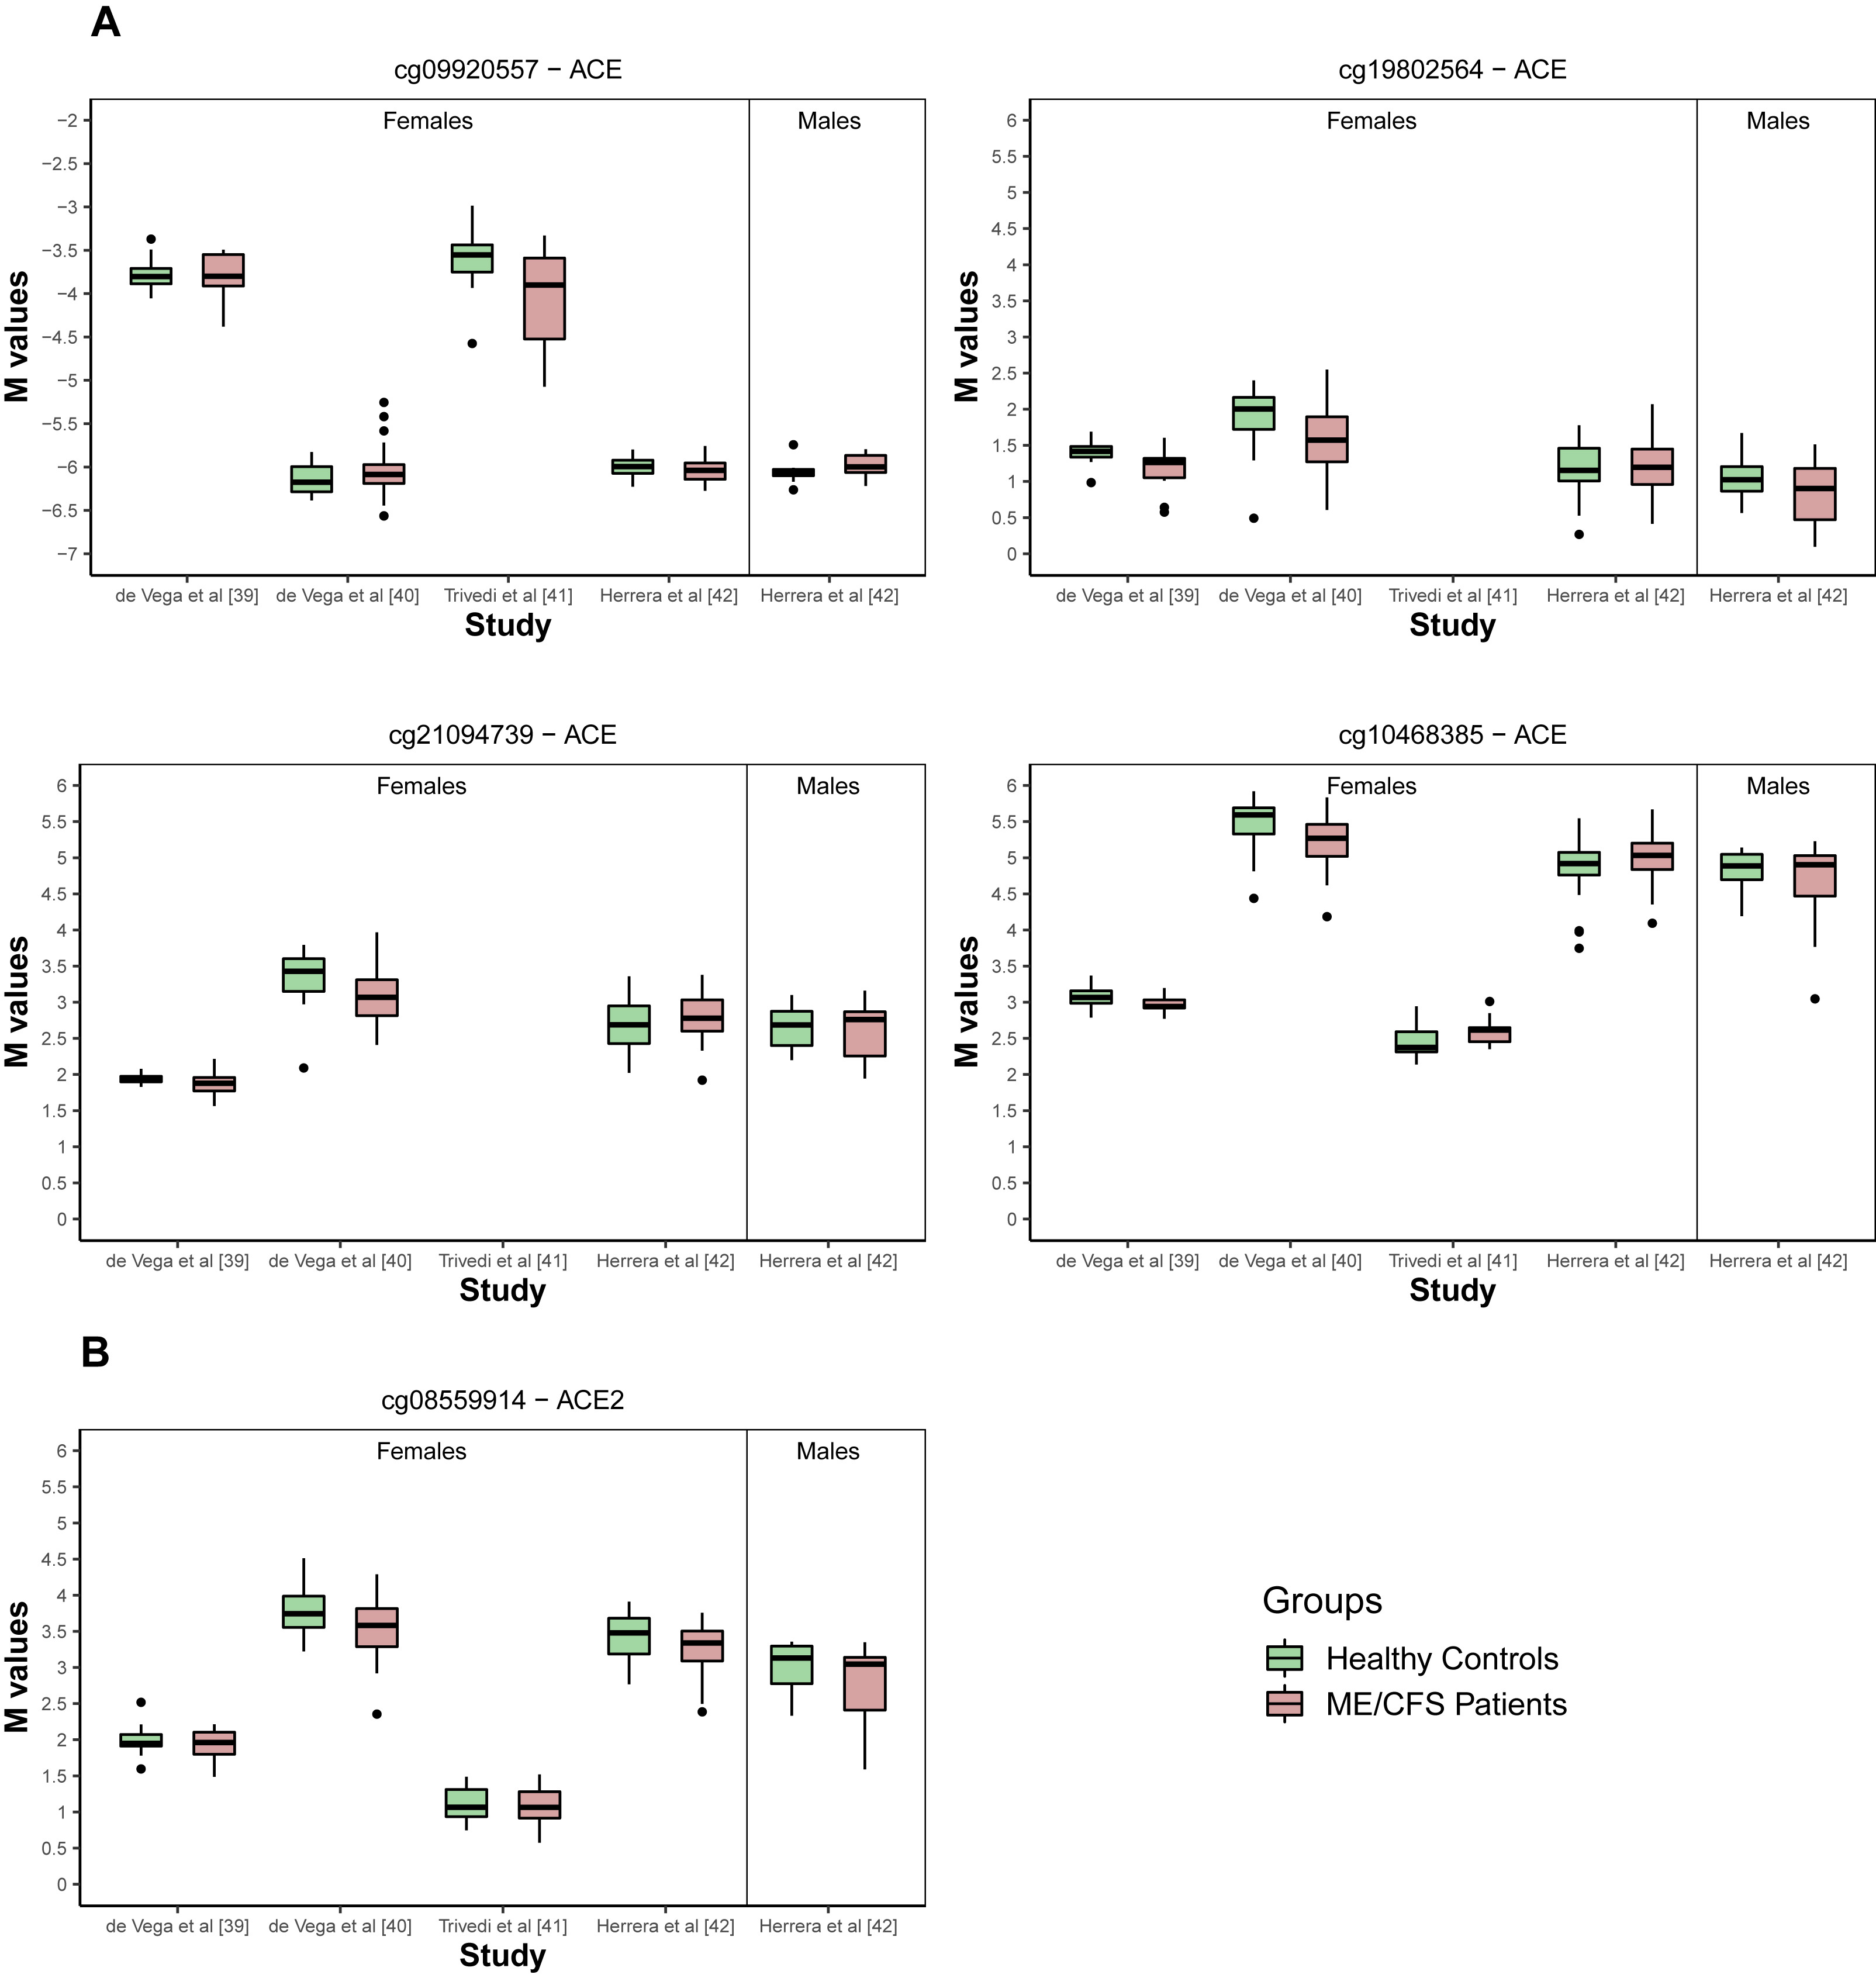
\includegraphics[width=0.9\textwidth]{chapter/2021-ace-ace2/figures/fig2-ace-ace2-mvalues.jpg}
    \caption[Boxplots per study, group and gender of the M-values referring to probes identified in Figure~\ref{fig:dna-methylation-analysis}C and Figure~\ref{fig:dna-methylation-analysis}D]{Boxplots per study, group and gender of the M-values referring to probes identified in Figure~\ref{fig:dna-methylation-analysis}C and Figure~\ref{fig:dna-methylation-analysis}D. (A) Significant probes located in \textit{ACE}. (B) Significant probe located in \textit{ACE2}.}
    \label{fig:ace-ace2-mvalues}
\end{figure}
% Figure 2
% Figure~\ref{fig:ace-ace2-mvalues}

Concerning the probes in \textit{ACE2}, the only significant association with ME/CFS was obtained for cg08559914 located in the TSS region of the gene (Figure~\ref{fig:dna-methylation-analysis}C). According to the best linear regression model for this probe, there was a negative association between the respective M-values and ME/CFS (coefficient estimate $= -0.141$ with a standard error of 0.048; Figure~\ref{fig:ace-ace2-mvalues}B and Supplementary Table~\ref{appendix:taba3-best-lm-models}). Given that a hypomethylated promoter region is typically indicative of an increased expression of the respective gene, this finding suggested an increased \textit{ACE2} expression in patients with ME/CFS.

We then repeated the same analysis for women and men separately. For women, we obtained the same disease associations, as described above (Figure~\ref{fig:dna-methylation-analysis}D and Supplementary Table~\ref{appendix:taba3-best-lm-models}). For men, we did not find any significant associations, probably due to data from a single study \citep{herrera2018GenomeepigenomeInteractions} (Figure~\ref{fig:dna-methylation-analysis}E).

%%%%%%%%%%%%%%%%%%%%%%%%%%%%%%%%%%%%%%%%%%%%%%%%%%%%%%%%%%%%%%%%%%%%%%%%
\subsection{Meta-analysis of ACE/ACE2 gene expression in ME/CFS patients}

We first conducted a re-analysis of the two studies in which the expression levels of \textit{ACE} or \textit{ACE2} were available for each participant (Figure~\ref{fig:ace-ace2-microarrays}A) \citep{saikiIdentificationMarkerGenes2008, gowGeneSignaturePostinfectious2009}. In the first study \citep{saikiIdentificationMarkerGenes2008}, there was evidence for an increased expression of \textit{ACE} in patients with ME/CFS (mean of the {$\log_{2}$}(fold-change) $= 0.$265; 95\% $\text{CI} = [0.089, 0.441]$). In the second study \citep{gowGeneSignaturePostinfectious2009}, the means of the {$\log_{2}$}(fold-change) were estimated at 0.012 (95\% $\text{CI} = [-0.012, 0.036]$) and 0.004 (95\% $\text{CI} = [-0.014, 0.022]$) for the two probes in \textit{ACE}. The corresponding estimates for the two probes in \textit{ACE2} were $-0.038$ (95\% $\text{CI}=[-0.085, 0.009]$) and $-0.037$ (95\% $\text{CI}=[-0.083, 0.008]$) (Figure~\ref{fig:ace-ace2-microarrays}A). The pooled estimates for this study were $0.007$ (95\% $\text{CI}=[-0.006, 0.020]$) and $-0.038$ (95\% $\text{CI}=[-0.067, -0.008]$) for \textit{ACE} and \textit{ACE2}, respectively.

Although not sharing the data, there was a study \citep{smithConvergentGenomicStudies2011} that reported a significant negative association between ME/CFS and \textit{ACE2} expression (see online Supplementary Table 2 of this study). In this case, we obtained the following mean of the {$\log_{2}$}(fold-change) $= -2.396$ and 95\% $\text{CI} = (-4.518, -0.273)$.

We then pooled the estimates from different studies for the same gene: $0.008$ (95\% $\text{CI}=[-0.005, 0.021]$) and $-0.038$ (95\% $\text{CI} = [-0.068, -0.009]$) for \textit{ACE} and \textit{ACE2}, respectively (Figure~\ref{fig:ace-ace2-microarrays}B). Therefore, our meta-analysis suggested a reduced expression of \textit{ACE2} but not of \textit{ACE} in patients with ME/CFS when comparing to healthy controls.

Finally, the remaining gene expression studies neither shared the respective data nor reported any differential \textit{ACE}/\textit{ACE2} expression between patients and healthy controls.

\begin{figure}
    \centering
    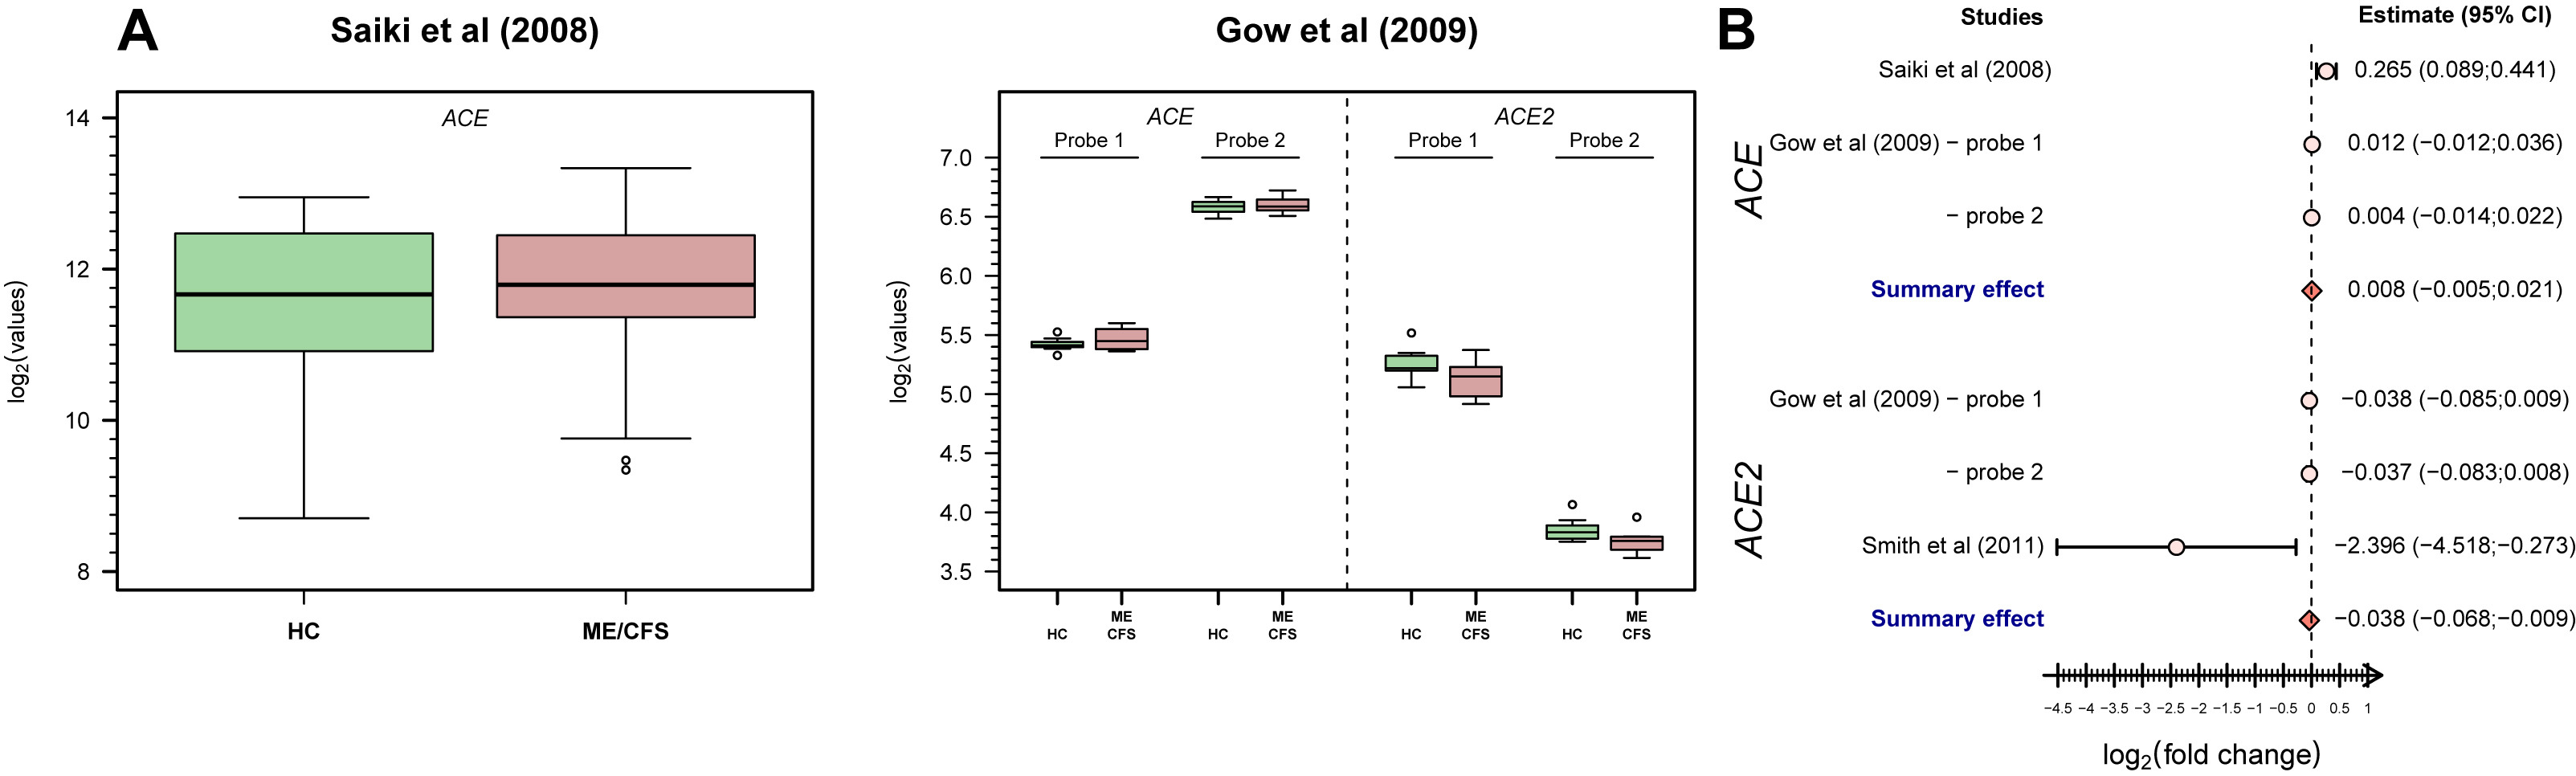
\includegraphics[width=0.95\textwidth]{chapter/2021-ace-ace2/figures/fig3-ace-ace2-microarrays.jpg}
    \caption[Analysis of \textit{ACE}/\textit{ACE2}-related data from eligible microarray-based gene expression studies]{Analysis of \textit{ACE}/\textit{ACE2}-related data from eligible microarray-based gene expression studies. (A) Boxplots of the data from these studies \citep{saikiIdentificationMarkerGenes2008, gowGeneSignaturePostinfectious2009}. (B) Forest plot for the study-specific and pooled estimate of the mean of the {$\log_{2}$}(fold-change) between patients with ME/CFS and healthy controls using data shown in A.}
    \label{fig:ace-ace2-microarrays}
\end{figure}
% Figure 3
% Figure~\ref{fig:ace-ace2-microarrays}

%%%%%%%%%%%%%%%%%%%%%%%%%%%%%%%%%%%%%%%%%%%%%%%%%%%%%%%%%%%%%%%%%%%%%%%%
\subsection{Analysis of ACE/ACE2 gene expression from a new female cohort}

To complement our findings from the above meta-analysis, we measured the \textit{ACE} and \textit{ACE2} mRNA levels in PBMCs from 37 women with ME/CFS (mean age $= 41.1$ years old) and 34 healthy women (mean age $= 37.4$ years old) (Table~\ref{tab:german-female-study}). Patients and healthy participants were matched for age (Kolmogorov-Smirnov test, p $= 0.38$). There was no information about the disease duration for 4 patients. The average disease duration for the remaining patients was 5.4 months in relation to the time of diagnosis (range $=$ 0--24 months).

\begin{table}[h]
    \centering
    \caption[Summary statistics for the gene expression of \textit{ACE} and \textit{ACE2} from the German female study participants]{Summary statistics for the gene expression of \textit{ACE} and \textit{ACE2} from the German female study participants where data of \textit{ACE2} were only available for 26 affected patients.}
    % \resizebox{\textwidth}{!}{% \begin{tblr}{
%  column{2} = {c},
%  column{3} = {c},
%  cell{4}{1} = {fg=MineShaft},
%  hline{1,11} = {-}{0.08em},
%  hline{2,5,8} = {-}{0.05em},
% }
% Summary statistic & Healthy controls & ME/CFS patients \\
% N & 34 & 37 \\
% Mean age (range), years & 37.4 (23; 65) & 41.1 (19; 60) \\
% {Mean disease duration since\\~diagnostic (range), months} & NA & 5.4 (0; 24) \\
% ACE & & \\
% Geometric mean & 0.153 & 0.144 \\
% Interquartile range & 0.087 & 0.073 \\
% ACE2 & & \\
% Geometric mean & 0.002 & 0.001 \\
% Interquartile range & 0.005 & 0.004 
% \end{tblr}
\begin{tabular}{lcc} 
\toprule
Summary statistic & Healthy controls & ME/CFS patients \\
\midrule
N & 34 & 37 \\
Mean age (range), years & 37.4 (23, 65) & 41.1 (19, 60) \\
\begin{tabular}[c]{@{}l@{}}Mean disease duration since\\~diagnostic (range), months\end{tabular} & --- & 5.4 (0, 24) \\
\midrule
ACE & & \\
~Geometric mean & 0.153 & 0.144 \\
~Interquartile range & 0.087 & 0.073 \\
\midrule
ACE2 & & \\
~Geometric mean & 0.002 & 0.001 \\
~Interquartile range & 0.005 & 0.004 \\ 
\bottomrule
\end{tabular}
% \cmidrule{3-5}
%  & & $n$ & Sample characteristics & Case definition & & & & \\ 
% \midrule
% % 1
% \citet{whistlerExerciseResponsiveGenes2005} & PBMC & 5 & \begin{tabular}[c]{@{}l@{}}Female adults\\Mean age: 42 years old\\Mean BMI: not reported\end{tabular} & CDC-1994 & 5 & \begin{tabular}[c]{@{}c@{}}Atlas Glass\\Human 3.8 I Microarray\\(BD Biosciences Clontech)\end{tabular} & No/No & No (NA) \\
% \midrule
% % 2
% \citet{kaushik2005GeneExpression} & PBMC & 25 & \begin{tabular}[c]{@{}l@{}}Female/male adults\\Mean age: 41 years old\\Mean BMI: not reported\end{tabular} & CDC-1994 & 25 & \begin{tabular}[c]{@{}c@{}}Custom microarray\\(Nimblegen)\end{tabular} & Unclear & No (NA) \\
% \midrule
% % 3
% \citet{kerr2008GeneExpression} & Whole blood & 25 & \begin{tabular}[c]{@{}l@{}}Female/male adults\\Mean age: 43 years old\\Mean BMI: not reported\end{tabular} & CDC-1994 & 50 & \begin{tabular}[c]{@{}c@{}}GeneChip\\Human Genome\\U133 Plus 2.0\\(Affymetrix)\end{tabular} & Yes/Yes & No (NA) \\
% \midrule
% % 4
% \citet{saikiIdentificationMarkerGenes2008} & Whole blood & 11 & \begin{tabular}[c]{@{}l@{}}Female/male adults\\Mean age: 34 years old\\Mean BMI: 20.3 kg/m\textsuperscript{2}\end{tabular} & CDC-1994 & 11 & \begin{tabular}[c]{@{}c@{}}Custom\\microarray (NA)\end{tabular} & Yes/No & Yes (NA){$^1$} \\
% \midrule
% % 5
% \citet{pietrangelo2009TranscriptionProfile} & Muscle biopsies & 4 & \begin{tabular}[c]{@{}l@{}}Female/male adults\\Mean age: 45/37 years old\\Mean BMI: not reported\end{tabular} & CDC-1994 & 5 & \begin{tabular}[c]{@{}c@{}}Operon V2.0\\(CRIBI\\University of Padova)\end{tabular} & Yes/Yes & No (NA) \\
% \midrule
% % 6
% \citet{gowGeneSignaturePostinfectious2009} & PBMC & \multicolumn{1}{l}{8} & \begin{tabular}[c]{@{}l@{}}Male adults\\Median age: 36 years old\\Mean BMI: not reported\end{tabular} & CDC-1994 & 7 & \begin{tabular}[c]{@{}c@{}}GeneChip\\Human Genome\\U133 (Affymetrix)\end{tabular} & Yes/Yes & Yes (GSE14577) \\
% \midrule
% % 7
% \citet{smithConvergentGenomicStudies2011} & PBMC & \multicolumn{1}{l}{37} & \begin{tabular}[c]{@{}l@{}}Female/male adults\\Mean age: 51 years old\\Mean BMI:29.4 kg/m\textsuperscript{2}\end{tabular} & CDC-1994 & 25 & \begin{tabular}[c]{@{}c@{}}MWG 20K\\human Array\\(Biotech MWG)\end{tabular} & Yes/Yes & No (NA) \\
% \midrule
% % 8
% \citet{jeffreyTreatmentAvenuesMyalgic2019} & PBMC & 33 & \begin{tabular}[c]{@{}l@{}}Female/male adults\\Mean age: not reported\\Mean BMI: not reported\end{tabular} & CDC-1994 & 21 & \begin{tabular}[c]{@{}c@{}}GeneChip\\Human Gene\\ST (Affymetrix)\end{tabular} & Yes/No & No (NA) \\
% \bottomrule
% \end{tabular}}
    % \begin{tblr}{
%  column{2} = {c},
%  column{3} = {c},
%  cell{4}{1} = {fg=MineShaft},
%  hline{1,11} = {-}{0.08em},
%  hline{2,5,8} = {-}{0.05em},
% }
% Summary statistic & Healthy controls & ME/CFS patients \\
% N & 34 & 37 \\
% Mean age (range), years & 37.4 (23; 65) & 41.1 (19; 60) \\
% {Mean disease duration since\\~diagnostic (range), months} & NA & 5.4 (0; 24) \\
% ACE & & \\
% Geometric mean & 0.153 & 0.144 \\
% Interquartile range & 0.087 & 0.073 \\
% ACE2 & & \\
% Geometric mean & 0.002 & 0.001 \\
% Interquartile range & 0.005 & 0.004 
% \end{tblr}
\begin{tabular}{lcc} 
\toprule
Summary statistic & Healthy controls & ME/CFS patients \\
\midrule
N & 34 & 37 \\
Mean age (range), years & 37.4 (23, 65) & 41.1 (19, 60) \\
\begin{tabular}[c]{@{}l@{}}Mean disease duration since\\~diagnostic (range), months\end{tabular} & --- & 5.4 (0, 24) \\
\midrule
ACE & & \\
~Geometric mean & 0.153 & 0.144 \\
~Interquartile range & 0.087 & 0.073 \\
\midrule
ACE2 & & \\
~Geometric mean & 0.002 & 0.001 \\
~Interquartile range & 0.005 & 0.004 \\ 
\bottomrule
\end{tabular}
% \cmidrule{3-5}
%  & & $n$ & Sample characteristics & Case definition & & & & \\ 
% \midrule
% % 1
% \citet{whistlerExerciseResponsiveGenes2005} & PBMC & 5 & \begin{tabular}[c]{@{}l@{}}Female adults\\Mean age: 42 years old\\Mean BMI: not reported\end{tabular} & CDC-1994 & 5 & \begin{tabular}[c]{@{}c@{}}Atlas Glass\\Human 3.8 I Microarray\\(BD Biosciences Clontech)\end{tabular} & No/No & No (NA) \\
% \midrule
% % 2
% \citet{kaushik2005GeneExpression} & PBMC & 25 & \begin{tabular}[c]{@{}l@{}}Female/male adults\\Mean age: 41 years old\\Mean BMI: not reported\end{tabular} & CDC-1994 & 25 & \begin{tabular}[c]{@{}c@{}}Custom microarray\\(Nimblegen)\end{tabular} & Unclear & No (NA) \\
% \midrule
% % 3
% \citet{kerr2008GeneExpression} & Whole blood & 25 & \begin{tabular}[c]{@{}l@{}}Female/male adults\\Mean age: 43 years old\\Mean BMI: not reported\end{tabular} & CDC-1994 & 50 & \begin{tabular}[c]{@{}c@{}}GeneChip\\Human Genome\\U133 Plus 2.0\\(Affymetrix)\end{tabular} & Yes/Yes & No (NA) \\
% \midrule
% % 4
% \citet{saikiIdentificationMarkerGenes2008} & Whole blood & 11 & \begin{tabular}[c]{@{}l@{}}Female/male adults\\Mean age: 34 years old\\Mean BMI: 20.3 kg/m\textsuperscript{2}\end{tabular} & CDC-1994 & 11 & \begin{tabular}[c]{@{}c@{}}Custom\\microarray (NA)\end{tabular} & Yes/No & Yes (NA){$^1$} \\
% \midrule
% % 5
% \citet{pietrangelo2009TranscriptionProfile} & Muscle biopsies & 4 & \begin{tabular}[c]{@{}l@{}}Female/male adults\\Mean age: 45/37 years old\\Mean BMI: not reported\end{tabular} & CDC-1994 & 5 & \begin{tabular}[c]{@{}c@{}}Operon V2.0\\(CRIBI\\University of Padova)\end{tabular} & Yes/Yes & No (NA) \\
% \midrule
% % 6
% \citet{gowGeneSignaturePostinfectious2009} & PBMC & \multicolumn{1}{l}{8} & \begin{tabular}[c]{@{}l@{}}Male adults\\Median age: 36 years old\\Mean BMI: not reported\end{tabular} & CDC-1994 & 7 & \begin{tabular}[c]{@{}c@{}}GeneChip\\Human Genome\\U133 (Affymetrix)\end{tabular} & Yes/Yes & Yes (GSE14577) \\
% \midrule
% % 7
% \citet{smithConvergentGenomicStudies2011} & PBMC & \multicolumn{1}{l}{37} & \begin{tabular}[c]{@{}l@{}}Female/male adults\\Mean age: 51 years old\\Mean BMI:29.4 kg/m\textsuperscript{2}\end{tabular} & CDC-1994 & 25 & \begin{tabular}[c]{@{}c@{}}MWG 20K\\human Array\\(Biotech MWG)\end{tabular} & Yes/Yes & No (NA) \\
% \midrule
% % 8
% \citet{jeffreyTreatmentAvenuesMyalgic2019} & PBMC & 33 & \begin{tabular}[c]{@{}l@{}}Female/male adults\\Mean age: not reported\\Mean BMI: not reported\end{tabular} & CDC-1994 & 21 & \begin{tabular}[c]{@{}c@{}}GeneChip\\Human Gene\\ST (Affymetrix)\end{tabular} & Yes/No & No (NA) \\
% \bottomrule
% \end{tabular}
    \label{tab:german-female-study}
\end{table}
% Table 3
% Table~\ref{tab:german-female-study}

We observed higher mRNA levels of \textit{ACE} than of \textit{ACE2} (Table~\ref{tab:results-bxcx-lm}, Figure~\ref{fig:mrna-correlation}A). There was no evidence for a significant correlation between \textit{ACE} and \textit{ACE2} expression levels (Spearman's correlation coefficient $= -0.120$) (Figure~\ref{fig:mrna-correlation}B). In contrast to the above meta-analysis, we could not find a reduced expression of \textit{ACE2} in patients with ME/CFS using the complete case scenario (Table~\ref{tab:results-bxcx-lm}). However, there were 11 (29.7\%) of the 37 samples from patients in which the expression level of \textit{ACE2} was below the limit of detection. This proportion of samples was significantly higher than that for healthy controls given that the expression of \textit{ACE2} could be quantified in all the samples (29.7\% versus 0\%; Pearson's $\chi^2$ test, p $= 0.002$). Consequently, we could not rule out that the patients with ME/CFS from this cohort have a decreased expression of \textit{ACE2} when compared to healthy controls. Finally, in accordance with our meta-analysis, there was no evidence of differential expression of \textit{ACE} between patients and healthy controls from this cohort.

\begin{table}[h]
    \centering
    \caption[Analysis of the linear regression models for the Box-Cox-transformed \textit{ACE} and \textit{ACE2} mRNA levels]{Analysis of the linear regression models for the Box-Cox-transformed \textit{ACE} and \textit{ACE2} mRNA levels where data were only available for 26 ME/CFS patients.}
    \begin{tblr}{
 column{2} = {r},
 column{3} = {r},
 hline{1,10} = {-}{0.08em},
 hline{2,6} = {-}{0.05em},
}
Analyses & Estimate (SE) & P-value \\
Box-Cox transformed ACE & & \\
\texttt{Intercept} & 0.541 (0.032) & $\leq 0.001$ \\
\texttt{Age} & 0.001 (0.001) & 0.328 \\
\texttt{Disease status (ME/CFS)} & $-$0.013 (0.018) & 0.481 \\
 % & & \\
Box-Cox transformed ACE2 & & \\
\texttt{Intercept} & 0.307 (0.038) & $\leq 0.001$ \\
\texttt{Age} & $-$0.001 (0.001) & 0.137 \\
\texttt{Disease status (ME/CFS)} & $-$0.006 (0.021) & 0.789 
\end{tblr}
    \label{tab:results-bxcx-lm}
\end{table}
% Table 4
% Table~\ref{tab:results-bxcx-lm}

\begin{figure}
    \centering
    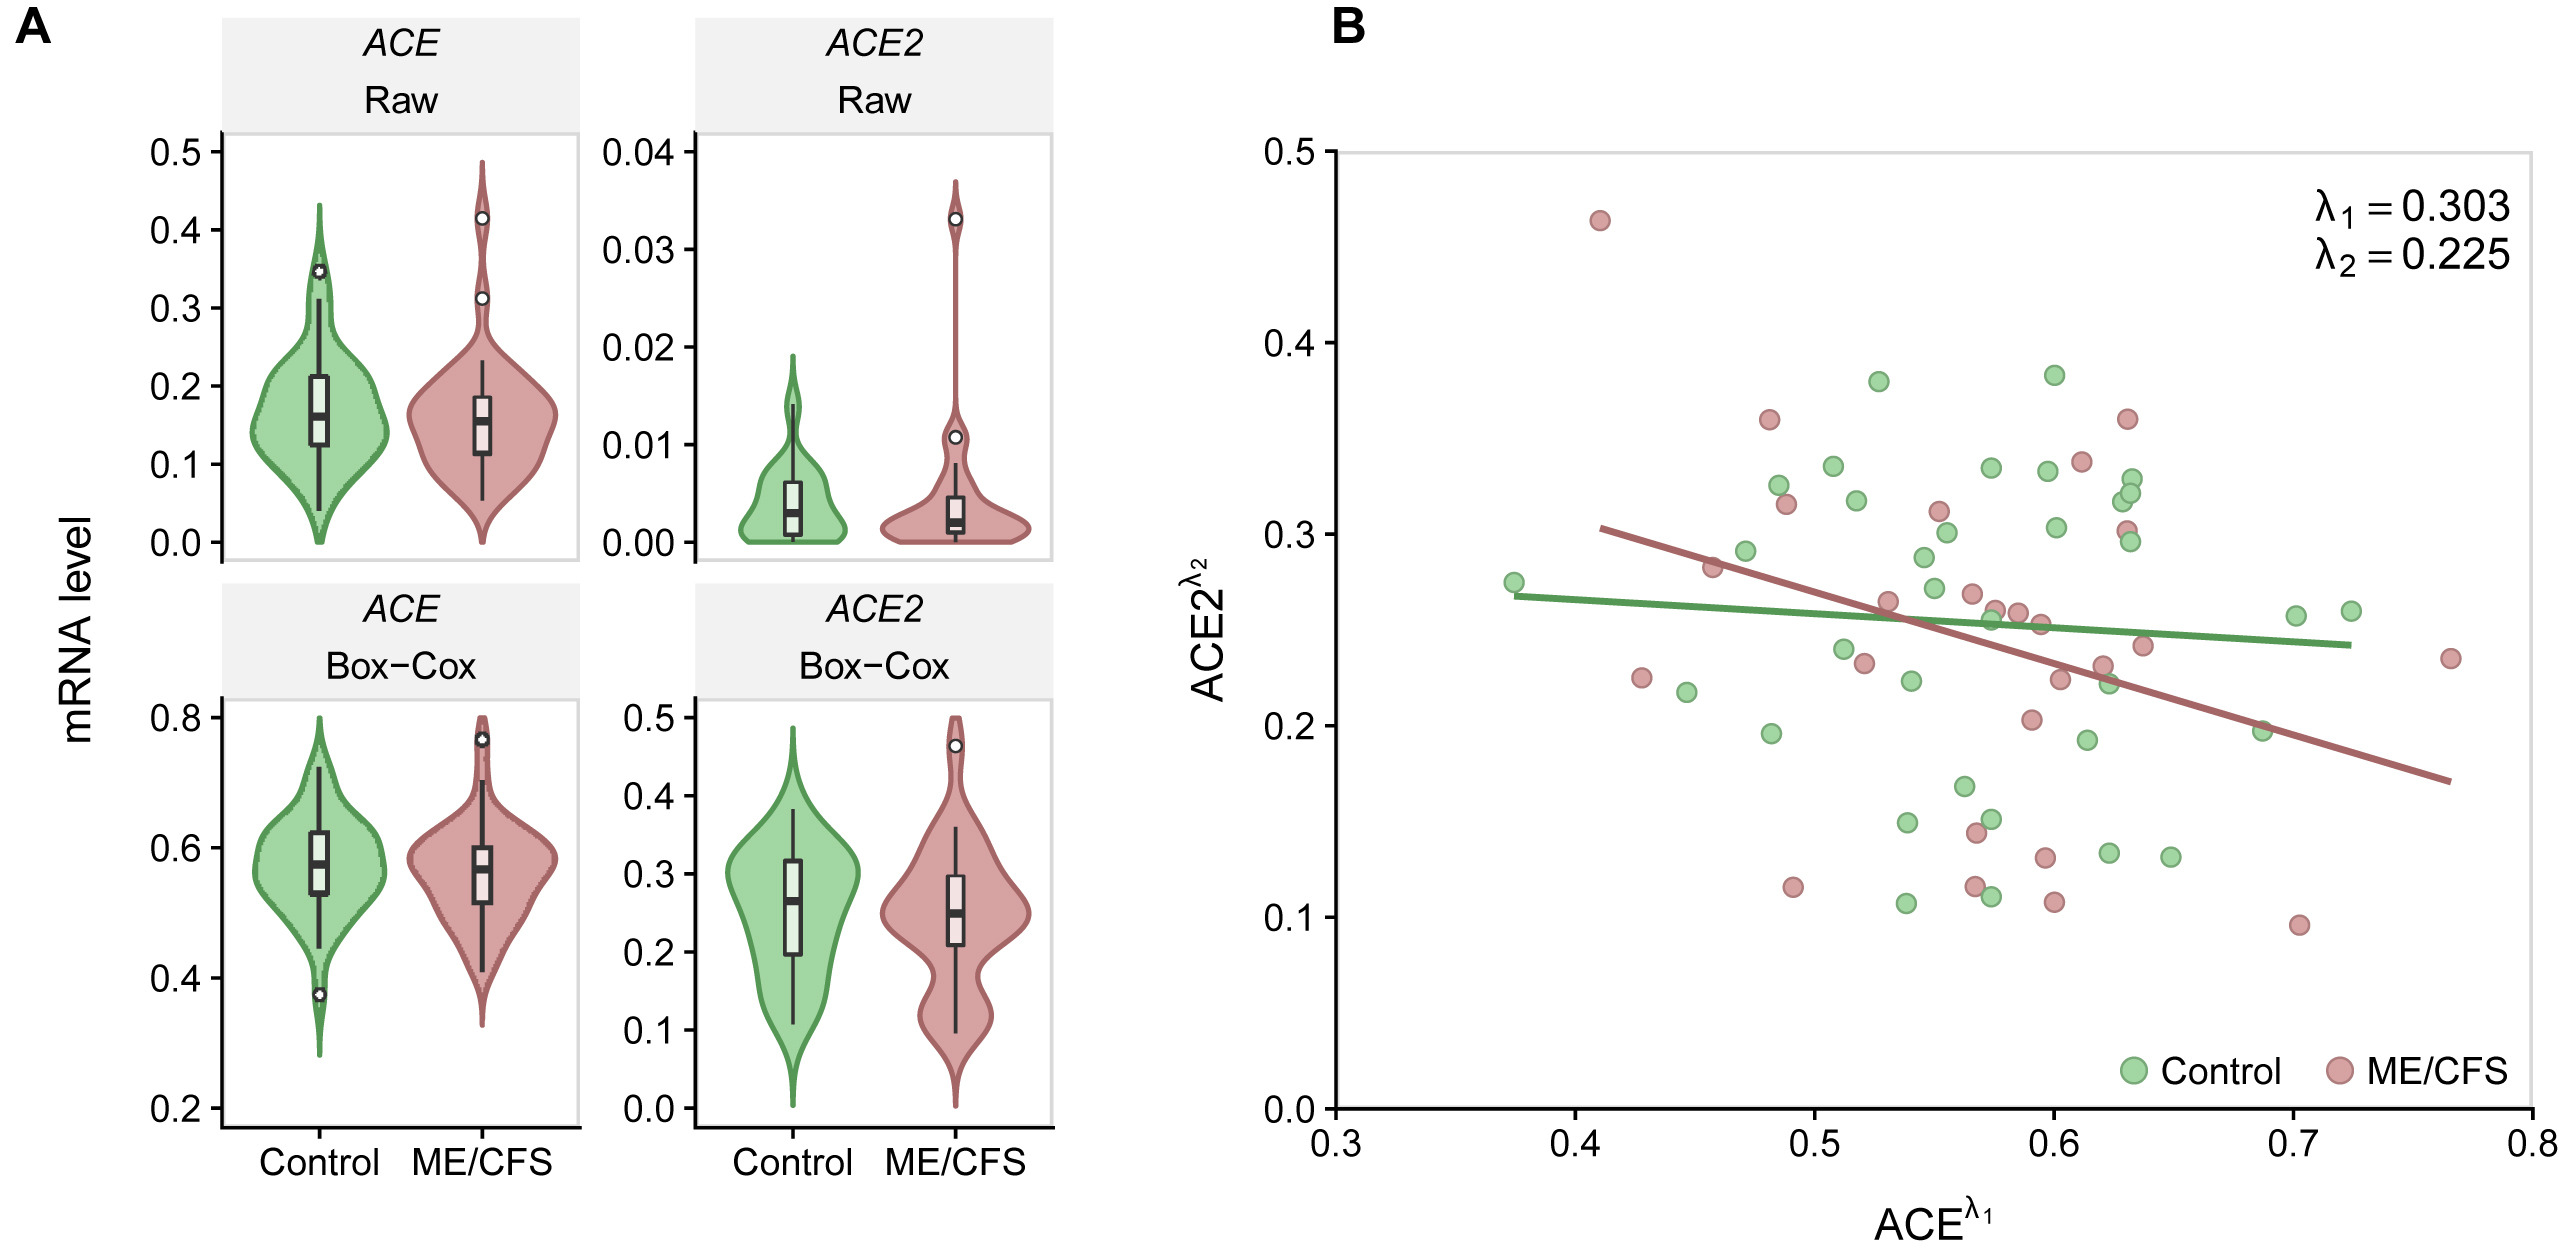
\includegraphics[width=\textwidth]{chapter/2021-ace-ace2/figures/fig4-mrna-correlation.jpg}
    \caption[Analysis of \textit{ACE} and \textit{ACE2} expression levels from the German study]{Analysis of \textit{ACE} and \textit{ACE2} expression levels from the German study. (A) Violin plots of \textit{ACE} (left side) and \textit{ACE2} (right side) mRNA raw data (upper row) and transformed data using a Box-Cox transformation (lower row). (B) Scatterplot between the transformed \textit{ACE} and \textit{ACE2} expression levels (Spearman's correlation coefficient $= -0.120$).}
    \label{fig:mrna-correlation}
\end{figure}
% Figure 4
% Figure~\ref{fig:mrna-correlation}

%%%%%%%%%%%%%%%%%%%%%%%%%%%%%%%%%%%%%%%%%%%%%%%%%%%%%%%%%%%%%%%%%%%%%%%%
%%%%%%%%%%%%%%%%%%%%%%%%%%%%%%%%%%%%%%%%%%%%%%%%%%%%%%%%%%%%%%%%%%%%%%%%
%%%%%%%%%%%%%%%%%%%%%%%%%%%%%%%%%%%%%%%%%%%%%%%%%%%%%%%%%%%%%%%%%%%%%%%%
\section{Discussion}

In this work, we investigated potential differences in \textit{ACE}/\textit{ACE2} DNA methylation and expression levels between patients with ME/CFS and healthy controls. With the identification of these differences, we expected to determine the health risk of patients with ME/CFS if infected by SARS-CoV-2. However, we stumbled upon hurdles related to (i) data unavailability for a possible re-analysis, (ii) availability of data derived from PBCMs and related subsets in which \textit{ACE2} is not particularly expressed, (iii) studies with unclear data quality, and (iv) studies using disease case definitions that are not recommended for research. As a consequence, we could not provide a more definite answer to our main research question.

Notwithstanding these difficulties, we could identify four CpG probes on \textit{ACE} and another one on \textit{ACE2} with decreased DNA methylation levels in patients with ME/CFS. This finding suggested an increased expression of the respective genes. However, our meta-analysis of public data suggested the opposite. Such decrease in \textit{ACE2} expression was partially confirmed by new data in which there was a significant higher proportion of samples below the limit of detection in patients with ME/CFS than in healthy controls. Nonetheless, it was clear that \textit{ACE2} is not particularly expressed in PBMCs from both patients with ME/CFS and healthy controls, as mentioned in the introduction.

In general, \textit{ACE2} downregulation is known to occur after host-cell entry by SARS-CoV-2 \citep{datta2020SARSCoV2Pandemic}. This downregulation is particularly problematic in individuals affected by cardiovascular diseases, diabetes, and other medical conditions, due to their low \textit{ACE2} levels before the infection \citep{verdecchia2020PivotalLink}. SARS-CoV-2 infection is then expected to further increase the ACE:ACE2 ratio, thus, promoting vasoconstriction, increased production of ROS and inflammation in patients with these co-morbidities \citep{pagliaro2020ACEACE2}. In this scenario, a putative reduction of the \textit{ACE2} expression makes patients with ME/CFS similar to these patients with a high risk for Covid-19. As a consequence, patients with ME/CFS could be considered a priority group for vaccination by public health authorities. The fundamental question is then to know whether our findings based on PBMCs could recreate what occurs in pulmonary epithelial and endothelial cells, the main targets of SARS-CoV-2. Future research should be conducted to answer this question, as similarly done in past studies aiming at understanding how the gene expression profiles from PBMCs could mimic those present in other tissues affecting by a given disease \citep{takamura2007GeneExpression, manoel-caetano2012GeneExpression, gerling2013GeneExpression}.

Given the residual \textit{ACE2} expression in PBMCs under normal conditions, one is tempted to say that SARS-CoV-2 does not infect these cells. However, earlier studies on SARS-CoV-1 found this virus within T lymphocytes, macrophages, and dendritic cells \citep{tay2020TrinityCOVID19}. More recently, an \textit{in vitro} study was able to infect PBMCs with SARS-CoV-2 \citep{codo2020ElevatedGlucose}. Monocytes are particularly susceptible to such infections. In this context, one cannot rule out that SARS-CoV-2 might use alternative receptors when infecting PBMCs.

Among the alternative receptors for SARS-CoV-2, the human transmembrane protease serine 2 (TMPRSS2) was suggested as a strong candidate \citep{sungnak2020SARSCoV2Entry} due to its role on SARS-CoV-1 infection \citep{matsuyama2010EfficientActivation, glowacka2011EvidenceThat}. This protease seems to induce SARS-CoV-2 cell entry through endocytosis via a mechanism of ACE2 cleavage \citep{hoffmann2020SARSCoV2Cell}. Another candidate receptor is the A disintegrin and metallopeptidase domain 17 protein (ADAM17) recognised by the immune system as a stress-response signal \citep{dusterhoft2019MetalloproteaseADAM17}. Like TMPRSS2, ADAM17 can also cleave ACE2 but with a reduced viral invasion efficiency \citep{heurich2014TMPRSS2ADAM17}.

With respect to the role of these proteases in ME/CFS, a targeted gene expression study analysed ADAM17 and other stress-response proteins \citep{saikiIdentificationMarkerGenes2008}. This study did not report any differential expression of this protease between patients with ME/CFS and healthy controls. However, this study is likely to be affected by a low statistical power due to small sample sizes for both groups. In addition, one of the selected DNA methylation studies suggested a decrease in the DNA methylation levels of one ADAM17-related CpG probe in patients with ME/CFS \citep{trivedi2018IdentificationMyalgic}.

Dipeptidyl peptidase-4 (DPP4), also known as the lymphocyte cell surface protein CD26, was found to be the main receptor for the Middle East respiratory syndrome–related coronavirus \citep{vandoremalen2014HostSpecies, widagdo2019SpeciesSpecificColocalization}. In contrast to ACE2, this surface protein is highly abundant in PBMCs including CD4\textsuperscript{+} and CD8\textsuperscript{+} T cells \citep{radzikowska2020DistributionACE2}. Bioinformatic analysis also suggested a strong interaction potential between this protein and SARS-CoV-2 \citep{li2020MERSCoVReceptor, vankadari2020EmergingWuHan}. Finally, DPP4 inhibitors were found to be protective against severe Covid-19 in patients with diabetes mellitus when compared to RAAS blockers \citep{rhee2021EffectsDPP4}. After initial concerns, this finding combined with others suggested an interesting therapeutic avenue against Covid-19 using DPP4 blockers \citep{scheen2021DPP4Inhibition}.

Interestingly, there is evidence for an increased proportion of natural killer cells and T cells expressing DPP4/CD26\textsuperscript{+} in patients with ME/CFS \citep{klimas1990ImmunologicAbnormalitiesa, fletcher2010BiomarkersChronic}. However, the number of DPP4/CD26 molecules was significantly reduced in T lymphocytes and natural killer cells of these patients \citep{fletcher2010BiomarkersChronic}. If DPP4 is indeed a relevant receptor for immune-cell invasion by SARS-CoV-2, research about this receptor should be prioritised when analysing PBMCs from patients with ME/CFS.

Sialic acids were also hypothesised as binding receptors used by SARS-CoV-2, as reported for other human coronaviruses \citep{sun2021RoleCell}. These acids are highly expressed in the epithelium cells of the lungs and oral cavity \citep{cross2018GlycanRecognition}. \textit{In vitro} and \textit{in silico} studies demonstrated the same binding potential for SARS-CoV-2 \citep{awasthi2020SialosideBindingPocket, baker2020SARSCOV2Spike, milanetti2021InSilicoEvidence}. However, the ACE2 glycosylation inhibition studies suggested that sialic acids on ACE2 receptor prevent ACE2-virus interaction \citep{chu2021HostViral, yang2020InhibitionSARSCoV2}. Again, detailed research on these putative receptors could help to determine the health risk of patients with ME/CFS when infected by SARS-CoV-2.

It was suggested that the arousal state experienced by patients with ME/CFS protects them against microbial infections \citep{sulheim2014DiseaseMechanisms}. This suggestion came from a clinical trial where patients were treated with clonidine to decrease such a state. Treated patients got their symptoms worsened and had their inflammation markers increased during the trial. In contrast, basic epidemiological studies reported many patients with frequent viral infections and flu-like symptoms \citep{johnston2016EpidemiologicalCharacteristics, chu2019OnsetPatterns, slomko2019PrevalenceCharacteristics}. The question is how an infection by SARS-CoV-2 lies in this contrasting evidence. A possible answer can be given with the assistance of the so-called sustained arousal model of ME/CFS \citep{wyller2009CanSustained}. According to this model, a sustained arousal state promotes in the long-run deleterious alterations of different body systems, including the immune system. Similar prediction was made by a recent study discussing the natural history of ME/CFS \citep{nacul2020HowMyalgic}. If so, patients with longer disease durations are more likely to show these immunological alterations than patients at the early stages of the disease. However, we could not analyse the effect of disease duration on our results, because this variable was not available in the public data sets included in our meta-analyses.

Finally, our original idea was also to include a meta-analysis of \textit{ACE}/\textit{ACE2} data from published genome-wide association studies on ME/CFS \citep{smithConvergentGenomicStudies2011, schlauch2016GenomewideAssociation, herrera2018GenomeepigenomeInteractions, perezGeneticPredispositionImmune2019, dibble2020GeneticRisk}. However, we could not materialise this idea, because such studies did not make their data publicly available. Nevertheless, evidence is scarce for a putative role of \textit{ACE}/\textit{ACE2} polymorphisms on ME/CFS. Two studies reported many candidate SNPs for such association, but none was located in \textit{ACE} or \textit{ACE2} \citep{smithConvergentGenomicStudies2011, schlauch2016GenomewideAssociation}. Two other studies did not find any significant SNPs associated with ME/CFS \citep{herrera2018GenomeepigenomeInteractions, dibble2020GeneticRisk}. The most optimistic study reported thousands of SNPs related to the disease \citep{perezGeneticPredispositionImmune2019}. However, this study did not perform all the basic quality control checks \citep{grabowska2020ReviewQuality}.

%%%%%%%%%%%%%%%%%%%%%%%%%%%%%%%%%%%%%%%%%%%%%%%%%%%%%%%%%%%%%%%%%%%%%%%%
%%%%%%%%%%%%%%%%%%%%%%%%%%%%%%%%%%%%%%%%%%%%%%%%%%%%%%%%%%%%%%%%%%%%%%%%
%%%%%%%%%%%%%%%%%%%%%%%%%%%%%%%%%%%%%%%%%%%%%%%%%%%%%%%%%%%%%%%%%%%%%%%%
\section{Conclusions}

Notwithstanding the low expression of \textit{ACE2} in PBMCs in general, there is evidence for a decreased expression of the gene in these cells from patients with ME/CFS. If PBMCs can qualitatively recreate what is occurring in the main cellular targets of SARS-CoV-2, then patients with this disease could be at a higher Covid-19 risk. In this regard, a recent preliminary report suggested that patients with ME/CFS got their symptoms worsened upon SARS-CoV-2 infection \citep{actionform.e.2021ReportImpact}. Altogether, these patients could be considered a priority group for vaccination against Covid-19, even though vaccines could trigger ME/CFS \citep{gherardi2019MyalgiaChronic, phelanPotentialAntigenicMimicry2020} or even exacerbate ME/CFS symptoms as the case of the natural immunisation by SARS-CoV-2. To further consolidate the existing evidence, future research should prioritise the collection of data from the main cellular targets in patients with ME/CFS. Further investigation should be also conducted on alternative SARS-CoV-2 receptors (i.e., DPP4 and sialic acids). At last, future research should also consider investigating putative sex differences in patients with ME/CFS given that, in general, men are more affected by Covid-19 than women \citep{gadi2020WhatSex}.
% \vfill
% \newpage

%%%%%%%%%%%%%%%%%%%%%%%%%%%%%%%%%%%%%%%%%%%%%%%%%%%%%%%%%%%%%%%%%%%%%%%%
\addcontentsline{toc}{section}{Bibliography}
\bibliographystyle{abbrvnat}
\bibliography{references}
%%%%%%%%%%%%%%%%%%%%%%%%%%%%%%%%%%%%%%%%%%%%%%%%%%%%%%%%%%%%%%%%%%%%%%%%

% Table 1
% Table~\ref{tab:methylation-studies}
% Table 2
% Table~\ref{tab:microarray-studies}
% Table 3
% Table~\ref{tab:german-female-study}
% Table 4
% Table~\ref{tab:results-bxcx-lm}

% Figure 1
% Figure~\ref{fig:dna-methylation-analysis}
% Figure 2
% Figure~\ref{fig:ace-ace2-mvalues}
% Figure 3
% Figure~\ref{fig:ace-ace2-microarrays}
% Figure 4
% Figure~\ref{fig:mrna-correlation}

% Supplementary Table 1
% Supplementary Table~\ref{appendix:taba1-ace-ace2-cpg-probes}
% Supplementary Table 2
% Supplementary Table~\ref{appendix:taba2-ace-ace2-cpg-polymorphic-probes}